\section{Desarrollo de Laboratorio}
\subsection{Ejercicio N° 01: Utilizando tablas temporales de auditoría}
\begin{itemize}  \item Paso 1 conecta esta ventana de consulta a tu copia de AdventureWorksLT
				 \item Paso 2 crear una tabla temporal versionada por el sistema
				 	
					\begin{center}
    				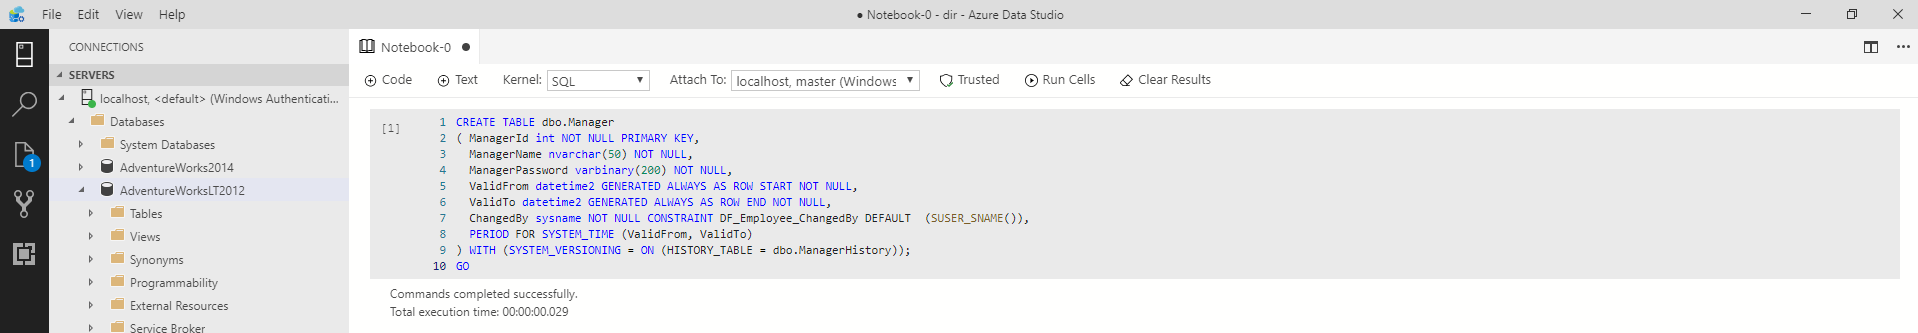
\includegraphics[width=16cm, height=90]{./Imagenes/Imagen1}
   				    \end{center}
				 

				 \item Paso 3 insertar datos de ejemplo
				 
				 	\begin{center}
    				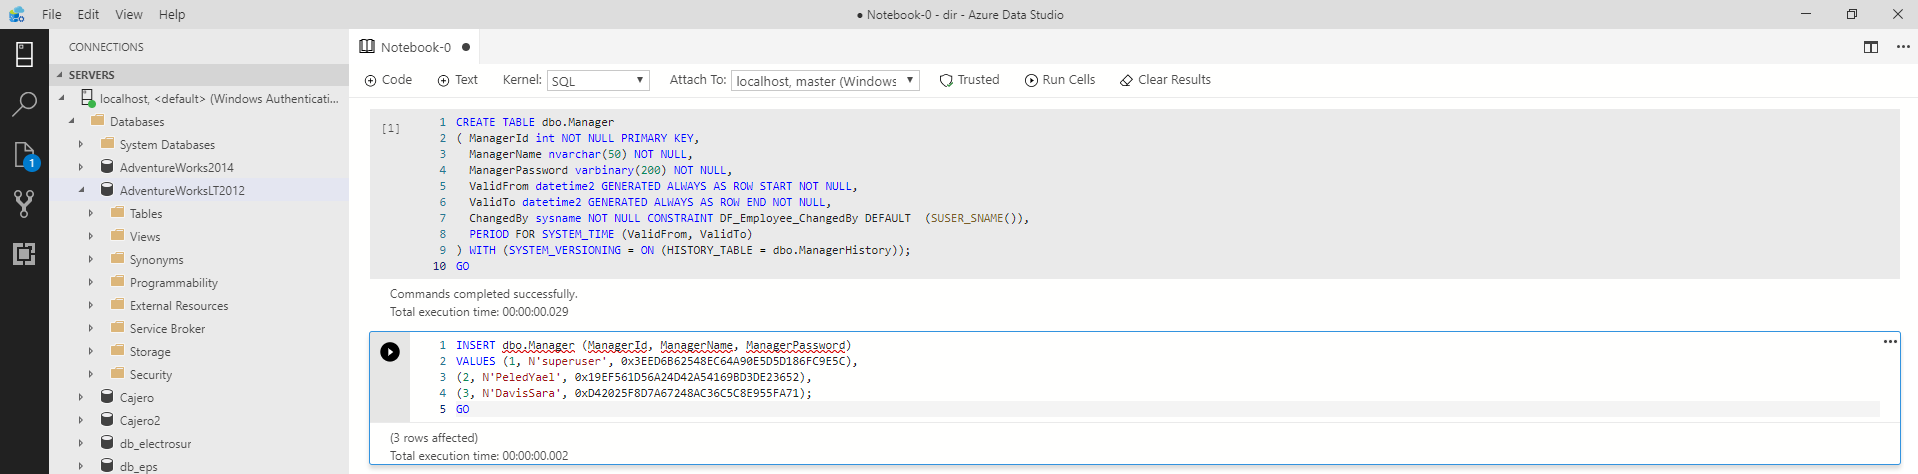
\includegraphics[width=16cm, height=90]{./Imagenes/Imagen2}
   				    \end{center}
				 
				 \item Paso 4 actualizar una fila
				 
				 
				 \begin{center}
    				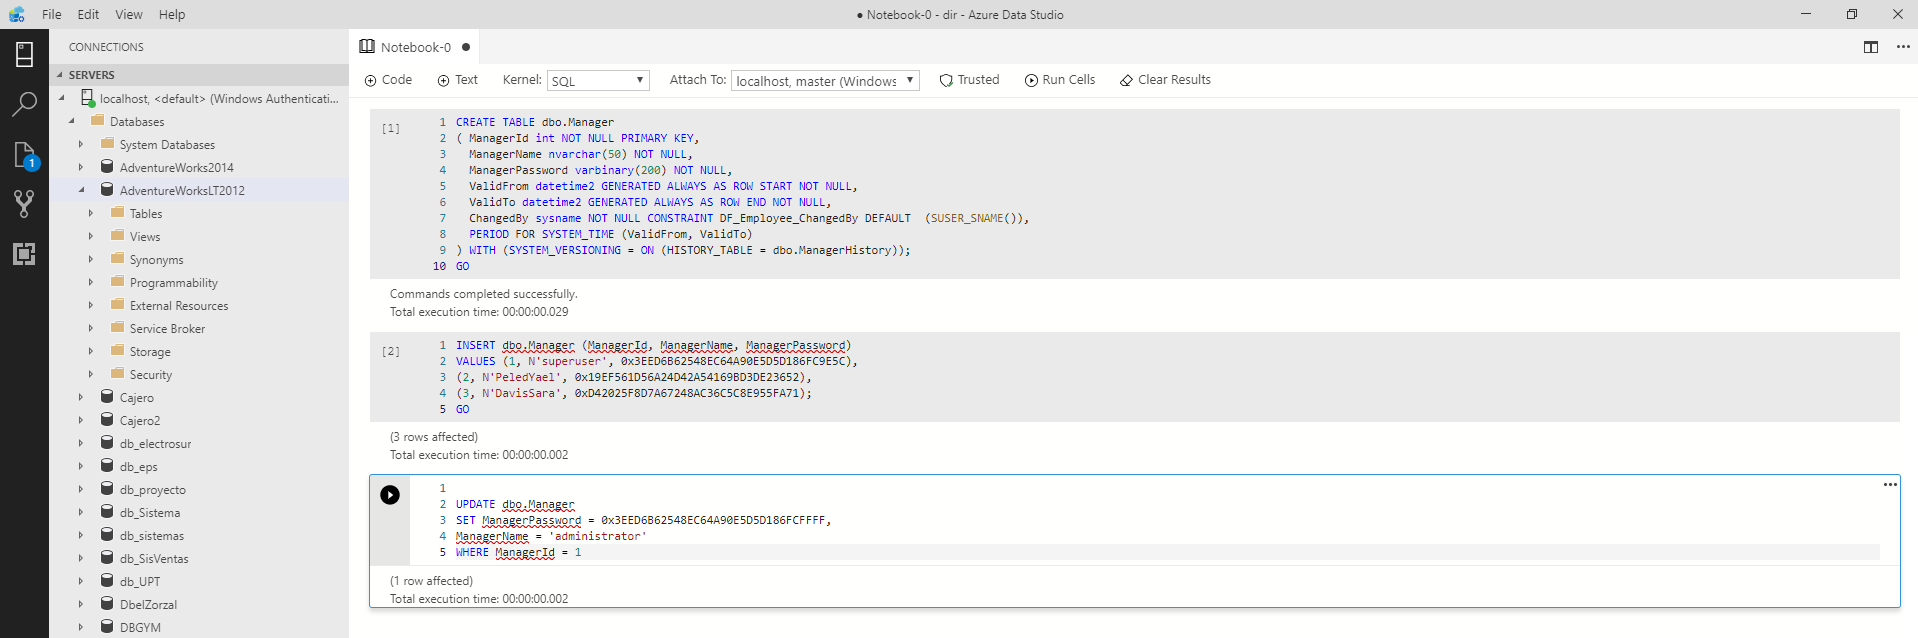
\includegraphics[width=16cm, height=90]{./Imagenes/Imagen3}
   				    \end{center}
				 
				 \item Paso 5 examinar tablas de componentes de la tabla temporal
				 
				 
				 \begin{center}
    				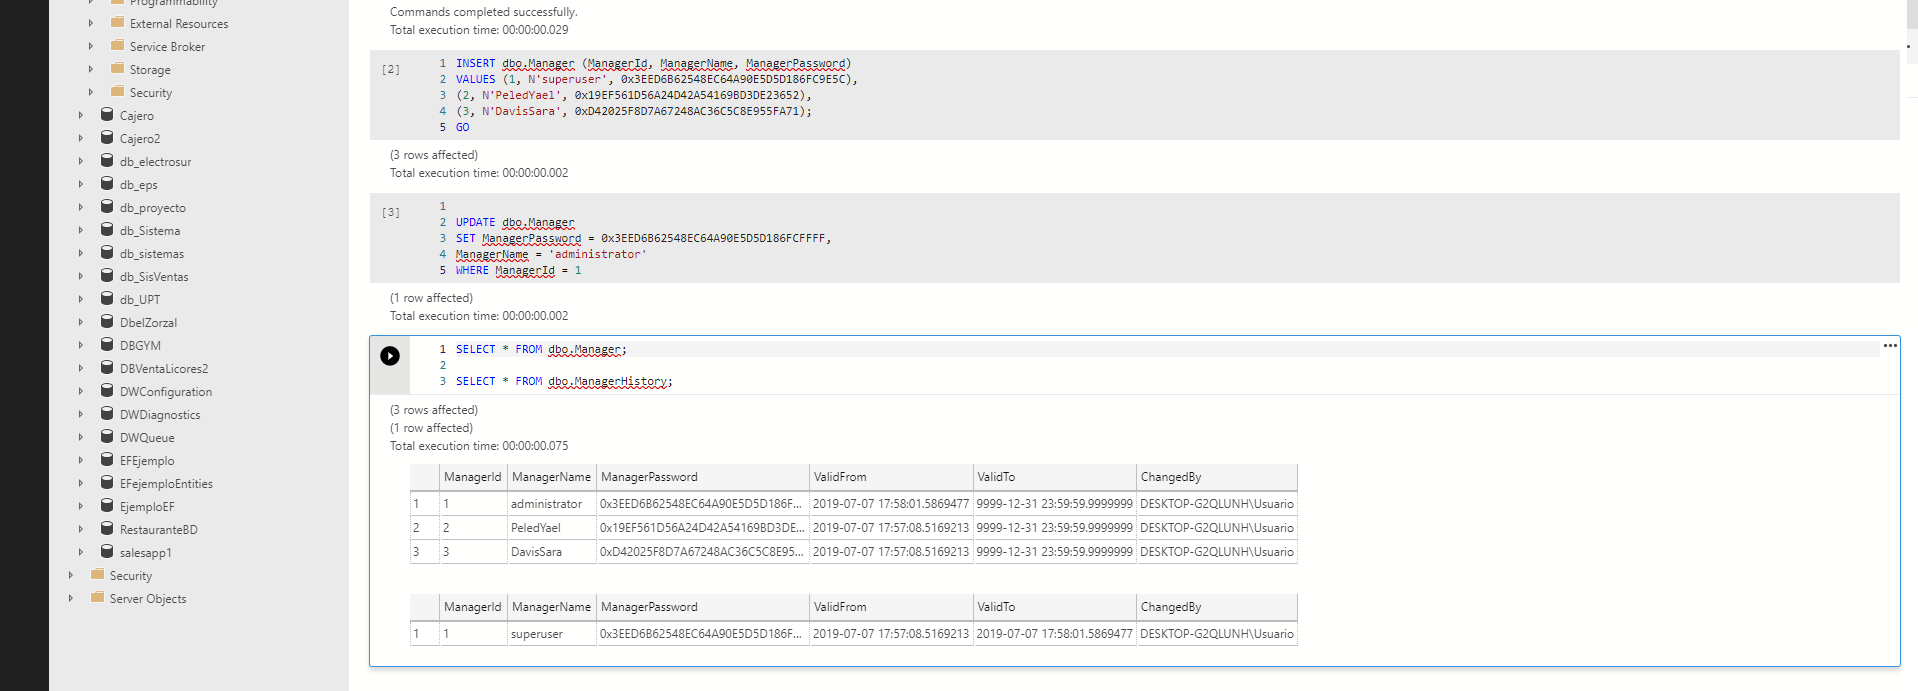
\includegraphics[width=16cm, height=90]{./Imagenes/Imagen4}
   				    \end{center}
   				    \clearpage		
   				    
   				 \item Paso 6 demuestre POR TODO EL TIEMPO DEL SISTEMA al consultar una tabla temporal TODOS muestra todos los datos en ambas tablas
				 
				 
				 \begin{center}
    				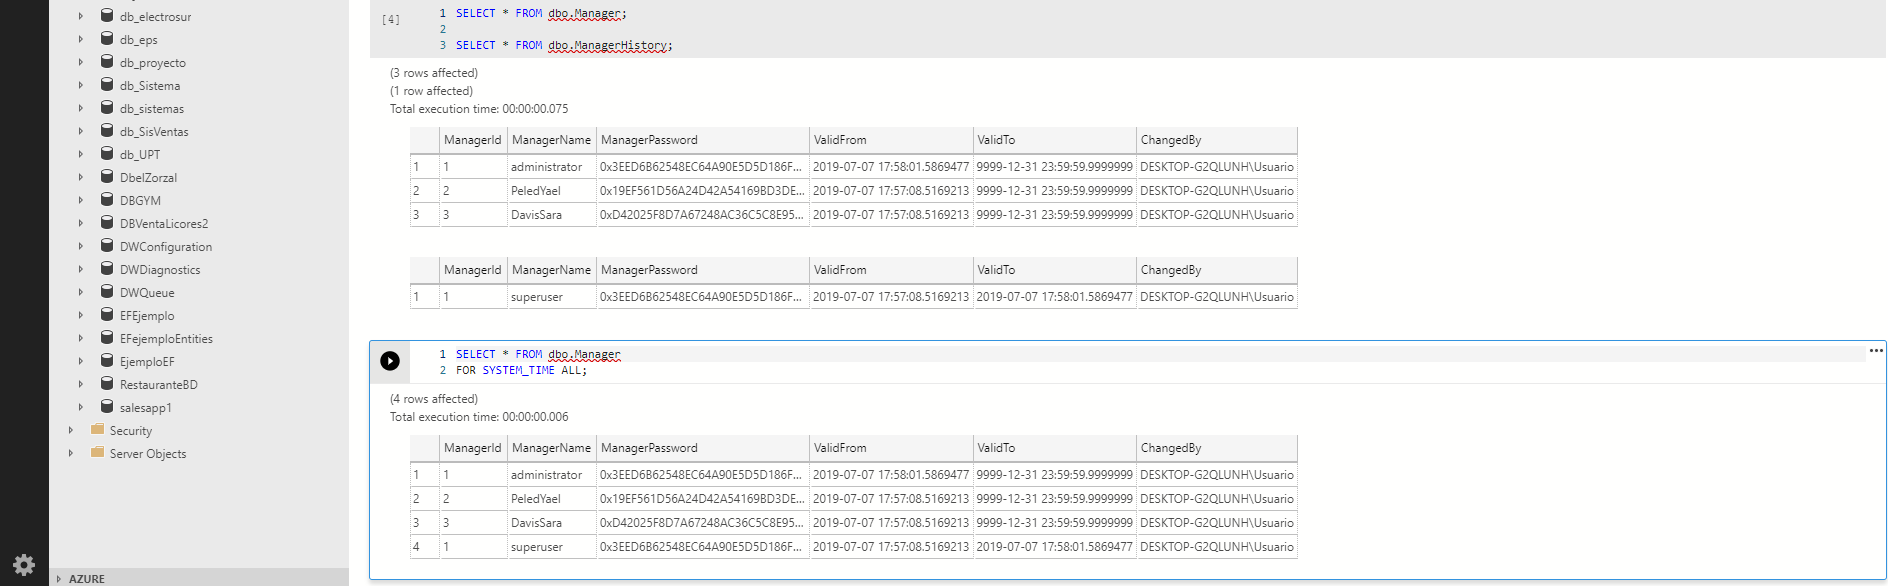
\includegraphics[width=16cm, height=90]{./Imagenes/Imagen5}
   				    \end{center}   		 
				 
				  \item Paso 7 demuestre POR TIEMPO DE SISTEMA COMO DE cuando se consulta una tabla temporal AS OF muestra un punto en el tiempo.
				 
				 \begin{center}
    				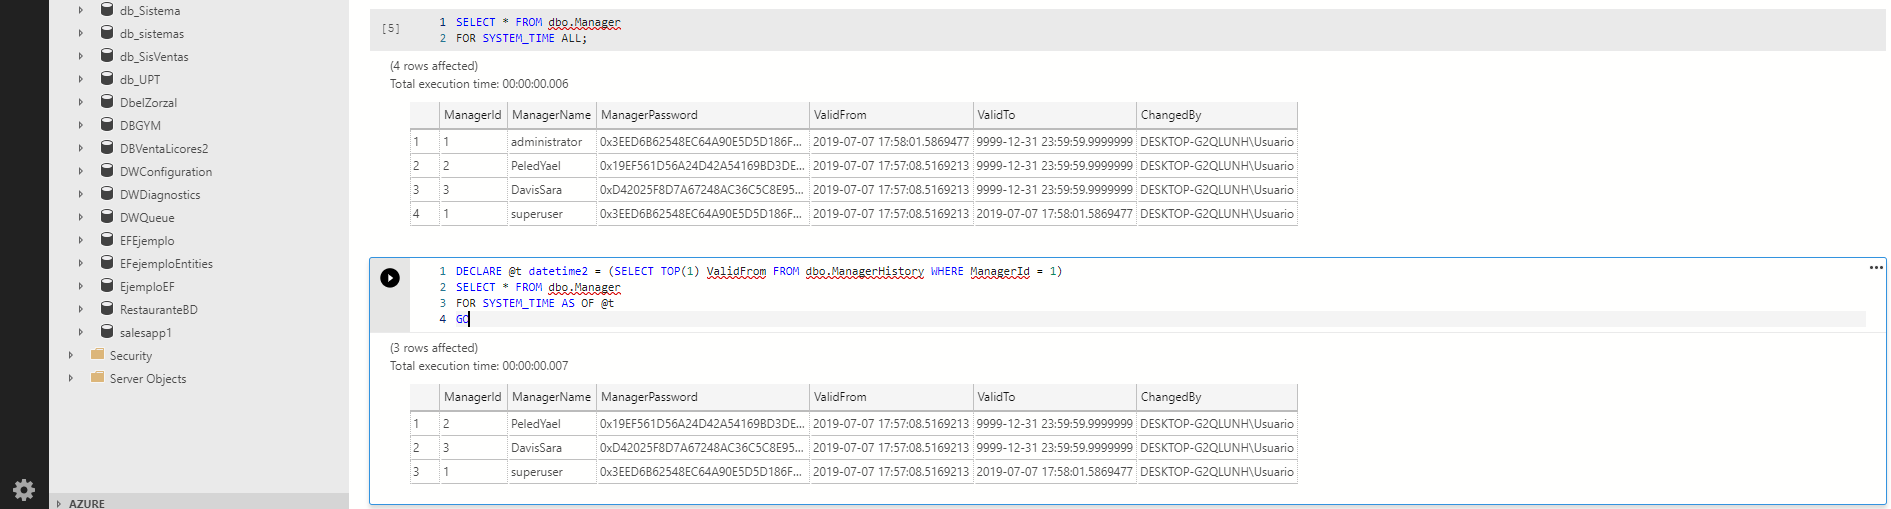
\includegraphics[width=16cm, height=90]{./Imagenes/Imagen6}
   				    \end{center} 
   				    
   				    \item Paso 8 demostrar que la tabla de historial no se puede editar (ambos comandos generarán un error)
				 
				 \begin{center}
    				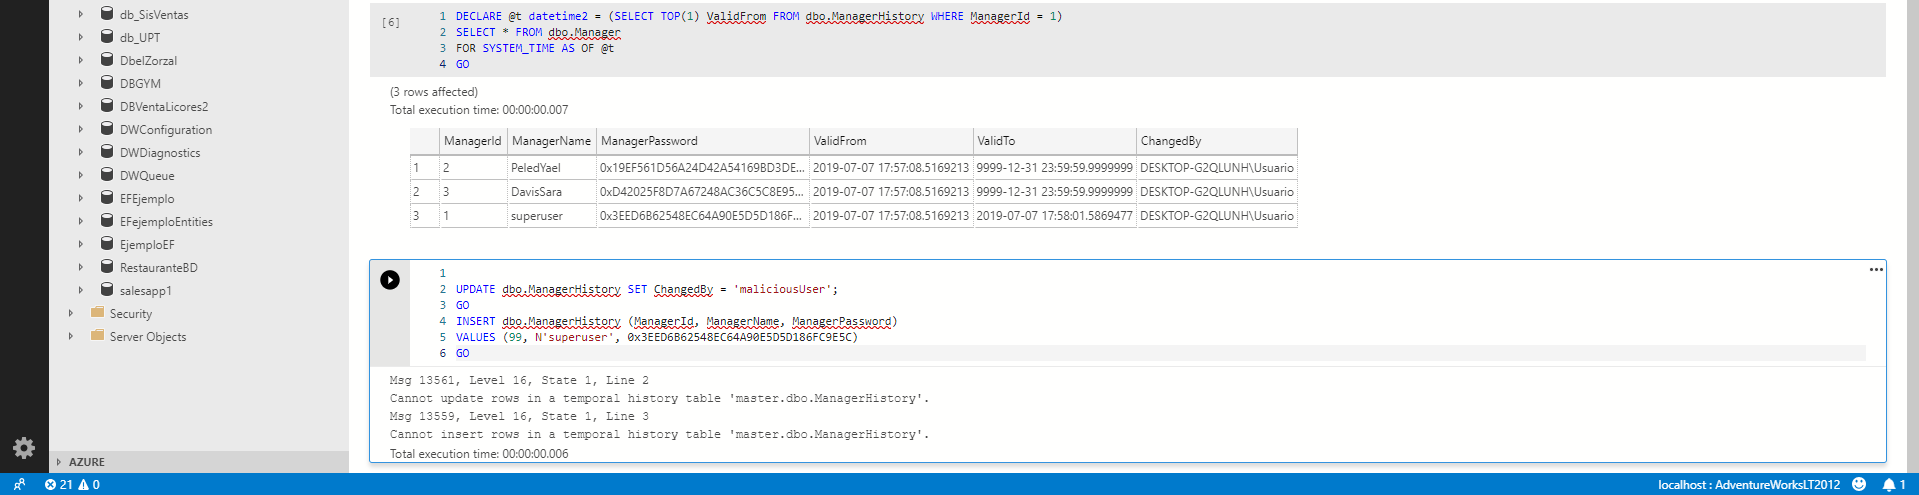
\includegraphics[width=16cm, height=90]{./Imagenes/Imagen7}
   				    \end{center}   
   				    
   				    \item Paso 9 demuestre que un usuario con permisos suficientes puede insertar datos engañosos en la columna ChangedBy:
				 
				 \begin{center}
    				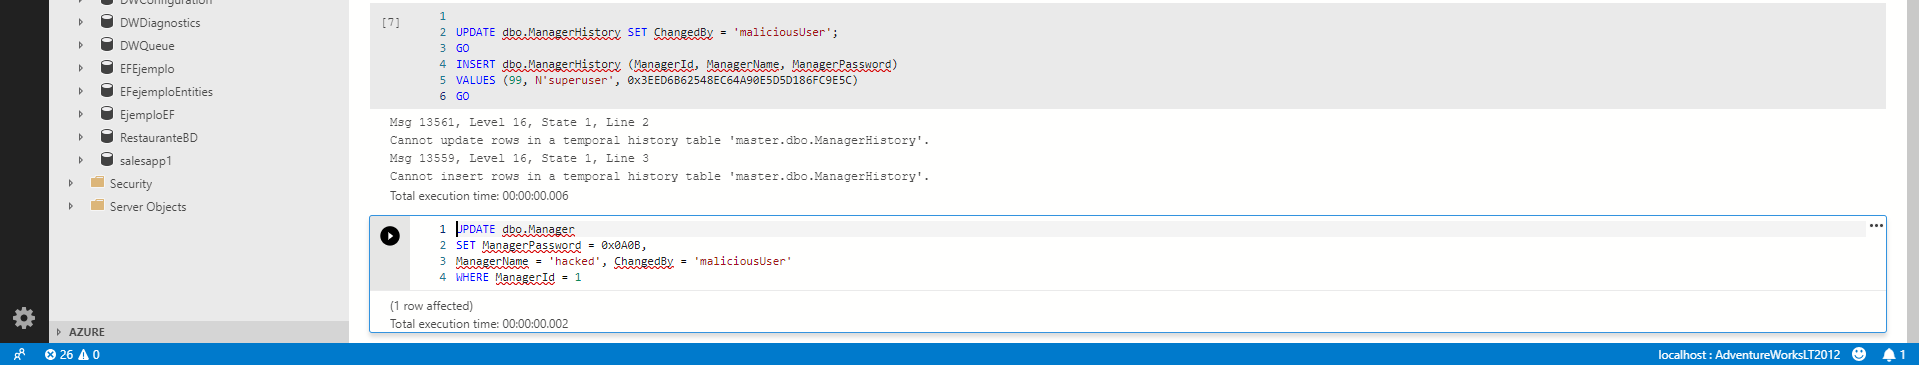
\includegraphics[width=16cm, height=90]{./Imagenes/Imagen8}
   				    \end{center}   
   				    \clearpage	
   				    \item Paso 10 examinar tablas de componentes de la tabla temporal
				 
				 \begin{center}
    				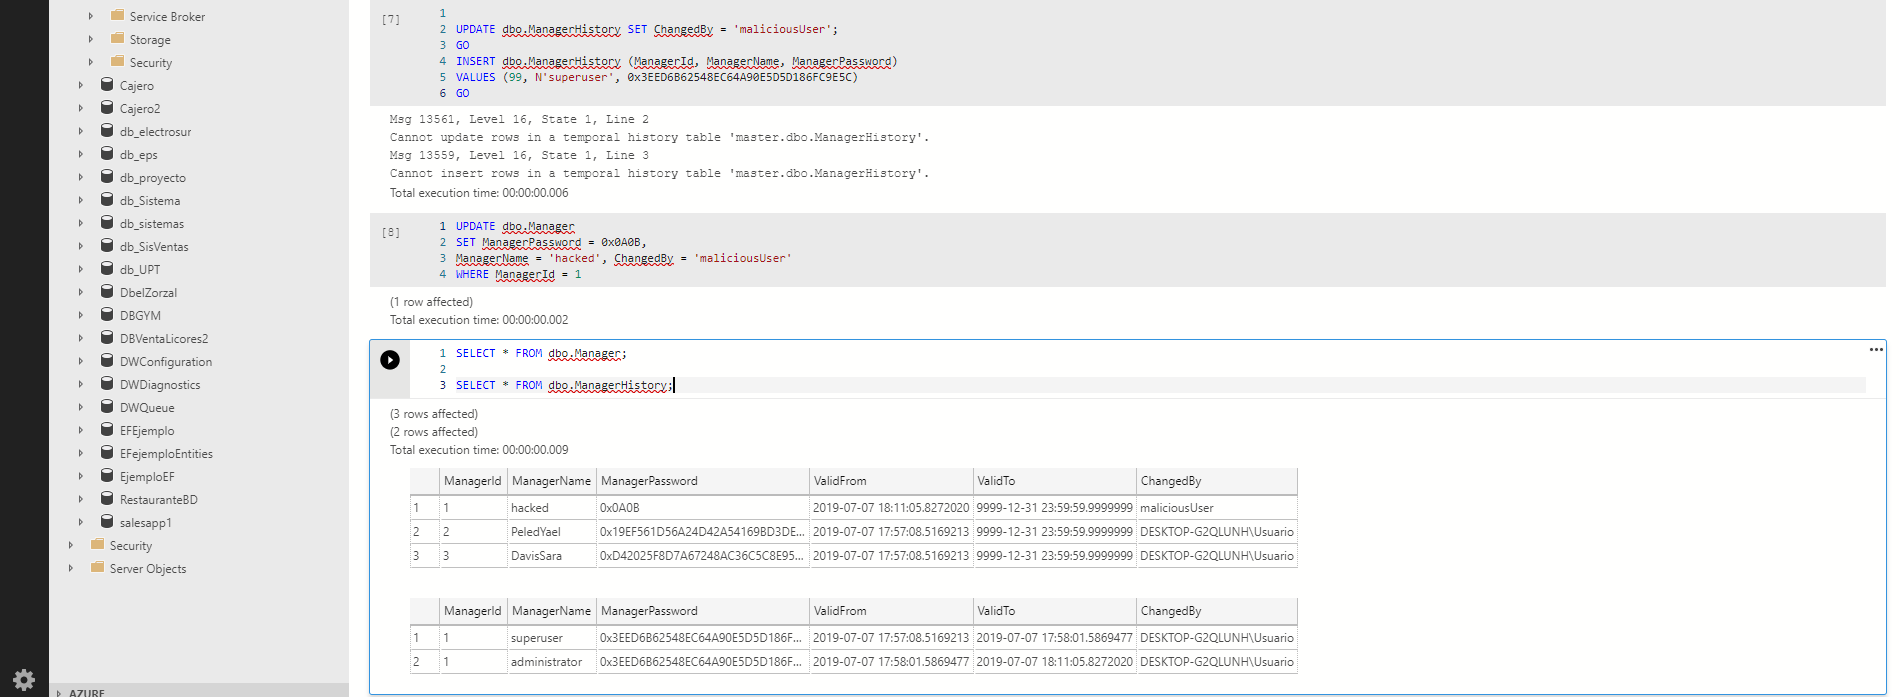
\includegraphics[width=16cm, height=90]{./Imagenes/Imagen9}
   				    \end{center} 	
   				    
   				     \item Paso 11 Cerrar objetos de demostración
				 
				 \begin{center}
    				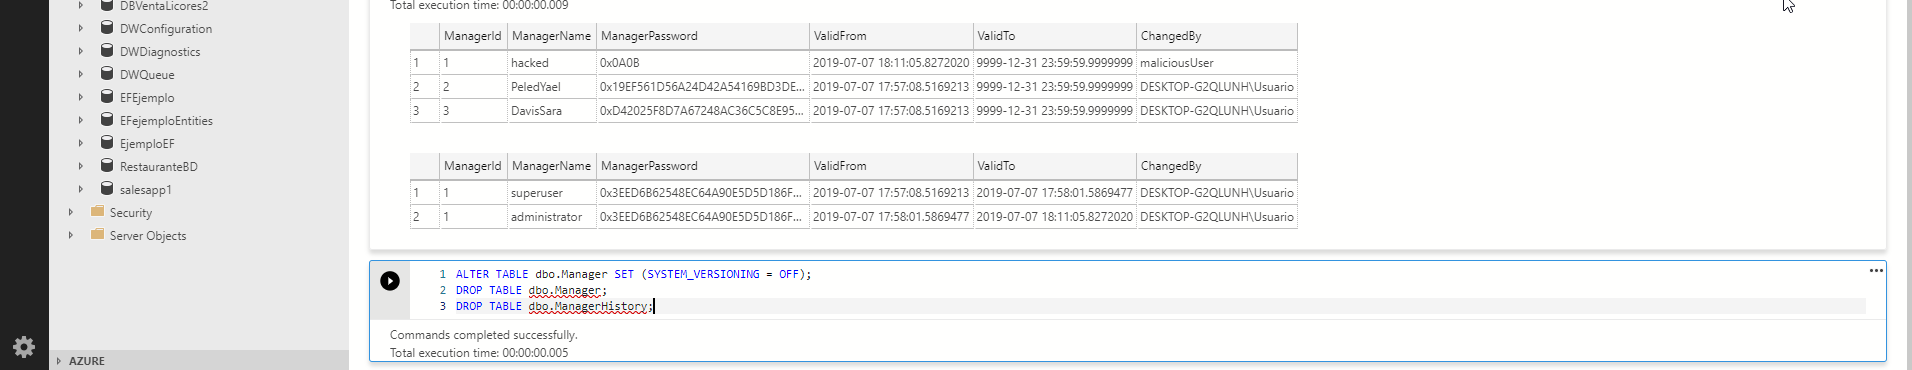
\includegraphics[width=16cm, height=90]{./Imagenes/Imagen10}
   				    \end{center} 		 
				 
				 
				 
				  
				 				  
				   \end{itemize}
				   \clearpage

\subsection{Ejercicio N° 02: Utilizando Auditorias}

			\begin{itemize}  
			
			\item Paso 1 Crear una auditoria
				 
				 	
					\begin{center}
    				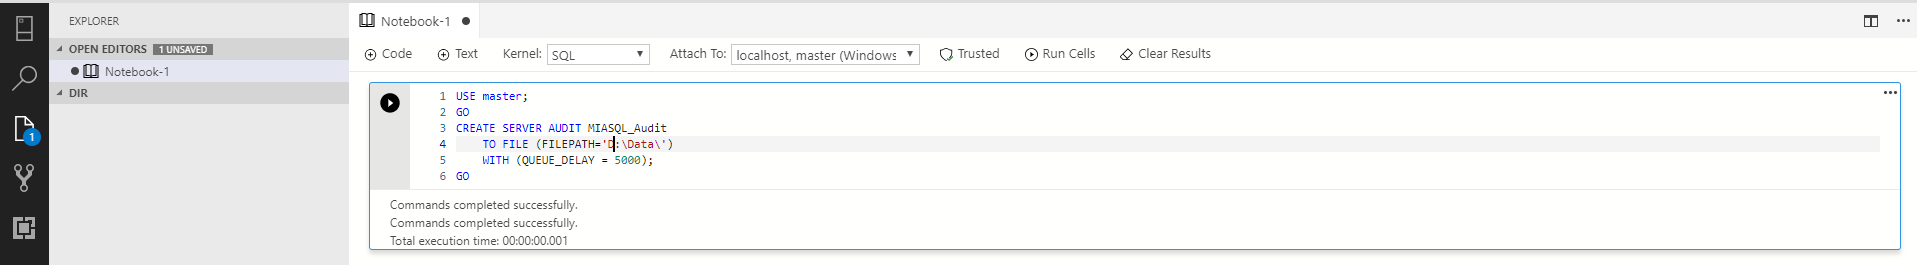
\includegraphics[width=16cm, height=90]{./Imagenes/Imagen_11}
   				    \end{center}
   				    
   				    \begin{center}
    				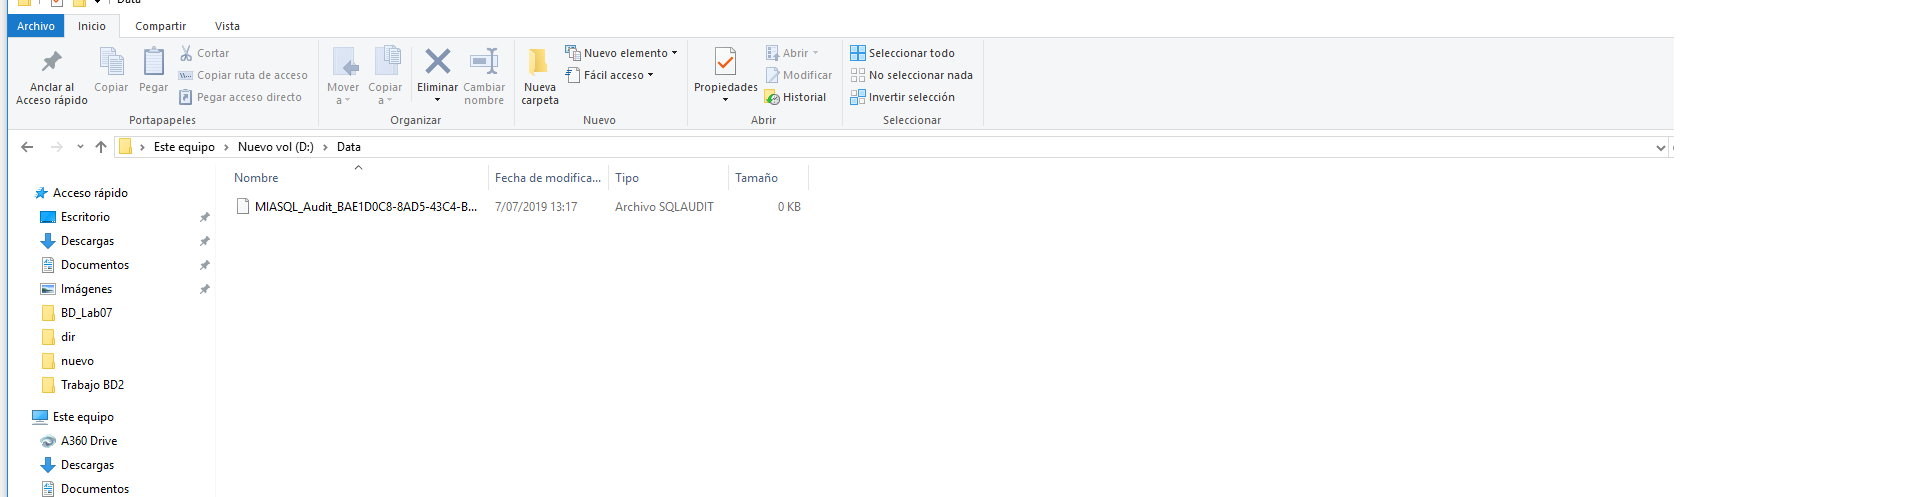
\includegraphics[width=16cm, height=90]{./Imagenes/AuditoriaCreada}
   				    \end{center}
   				    
   		   \item Paso 2 Habilitar la auditoria
				 
				 	
					\begin{center}
    				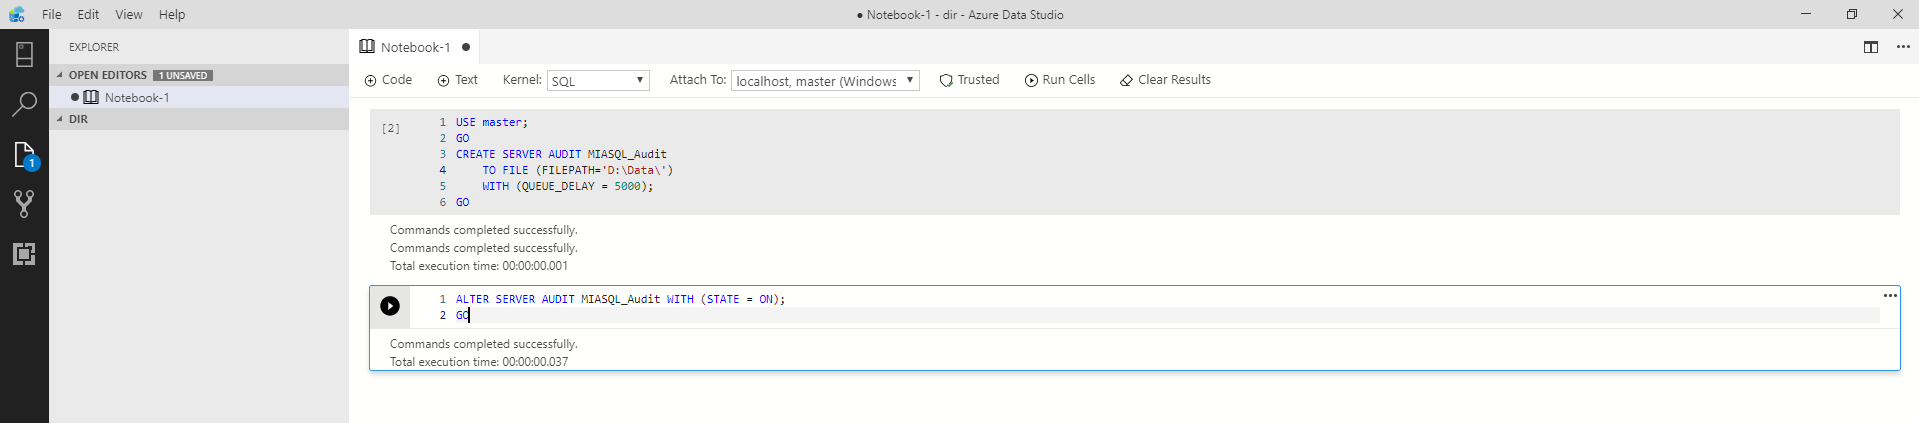
\includegraphics[width=16cm, height=90]{./Imagenes/Imagen_12}
   				    \end{center}
   				    
   		   \item Paso 3 Crear una especificación de auditoría del servidor
				 
				 	
					\begin{center}
    				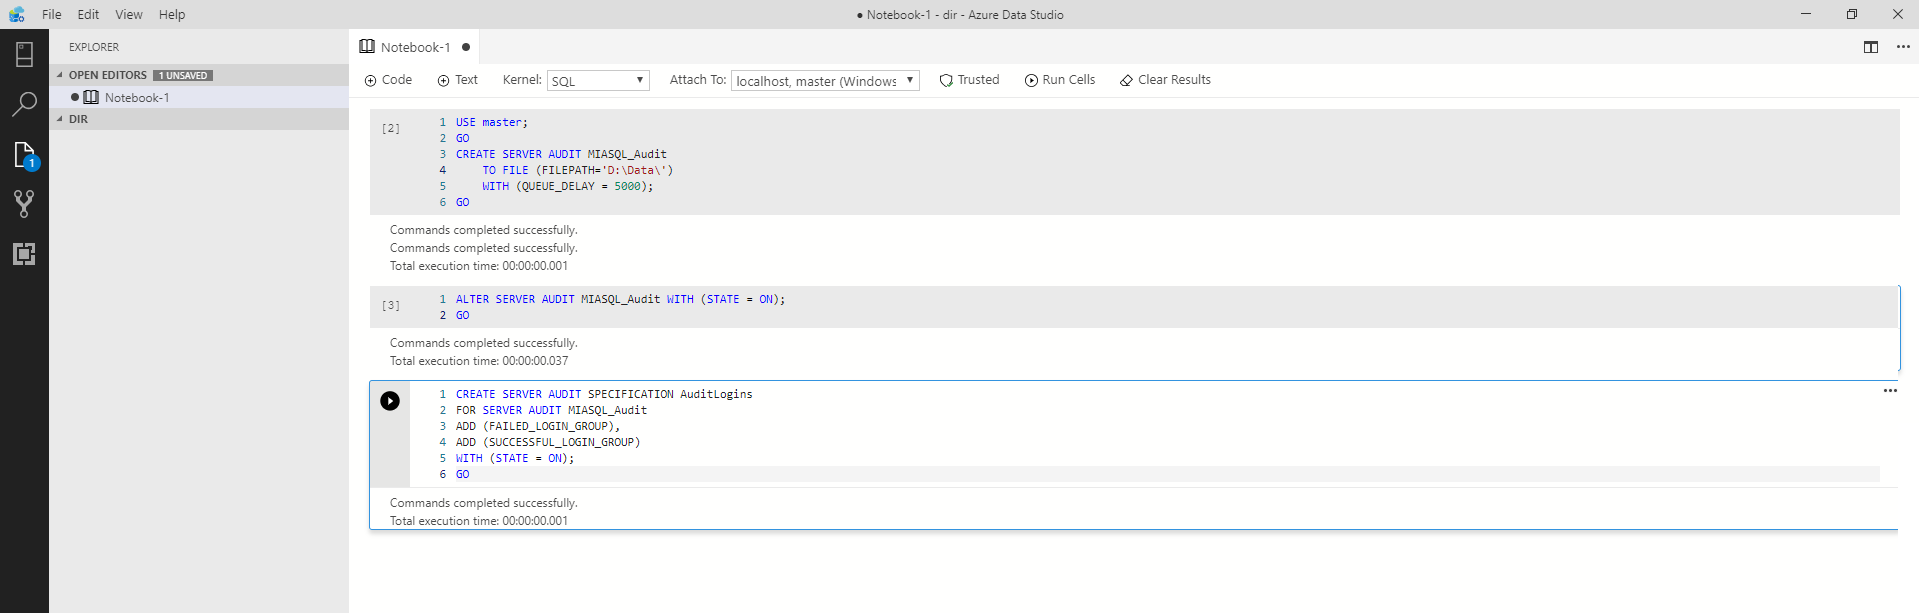
\includegraphics[width=16cm, height=90]{./Imagenes/Imagen_13}
   				    \end{center}
   				    
   		   \item Paso 4 Crear una especificación de auditoría de base de datos
				 
				 	
					\begin{center}
    				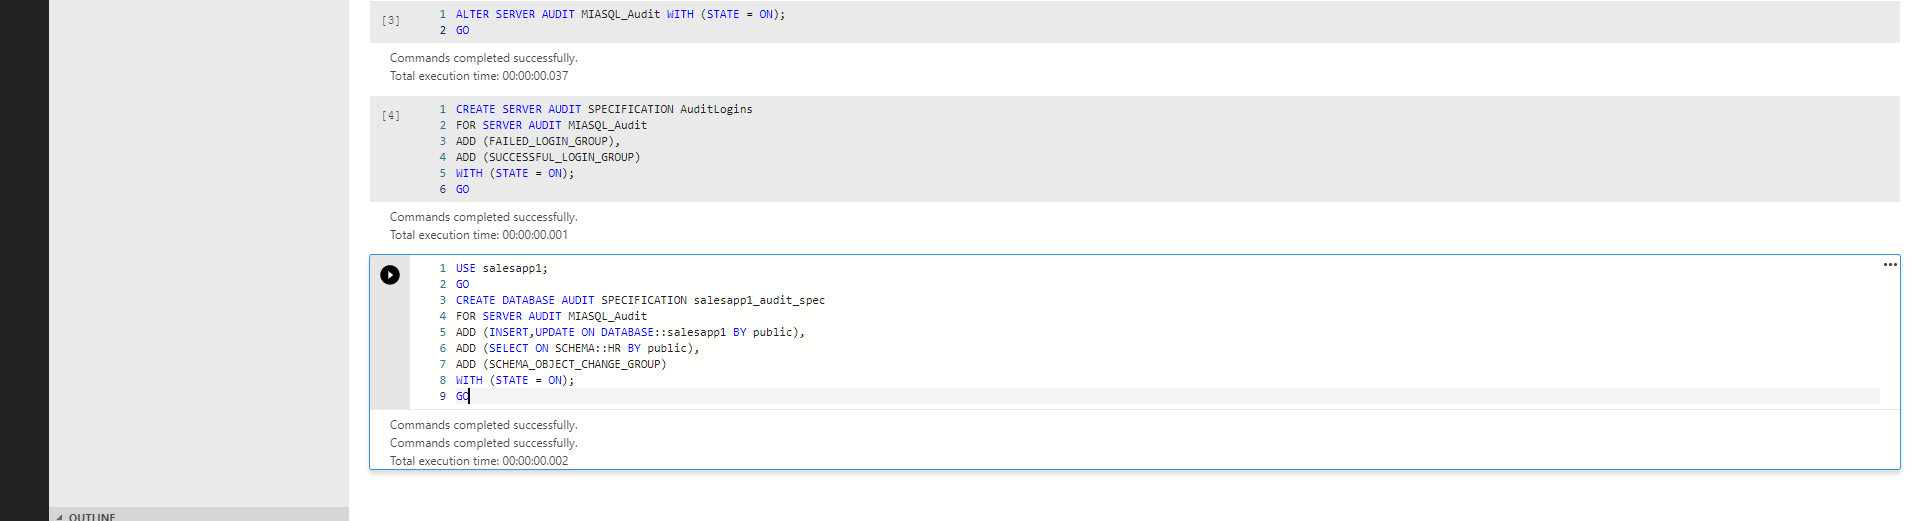
\includegraphics[width=16cm, height=90]{./Imagenes/Imagen_14}
   				    \end{center}
   				    
   		  \item Paso 5 Alterar la especificación de auditoría de la base de datos
				 
				 	
					\begin{center}
    				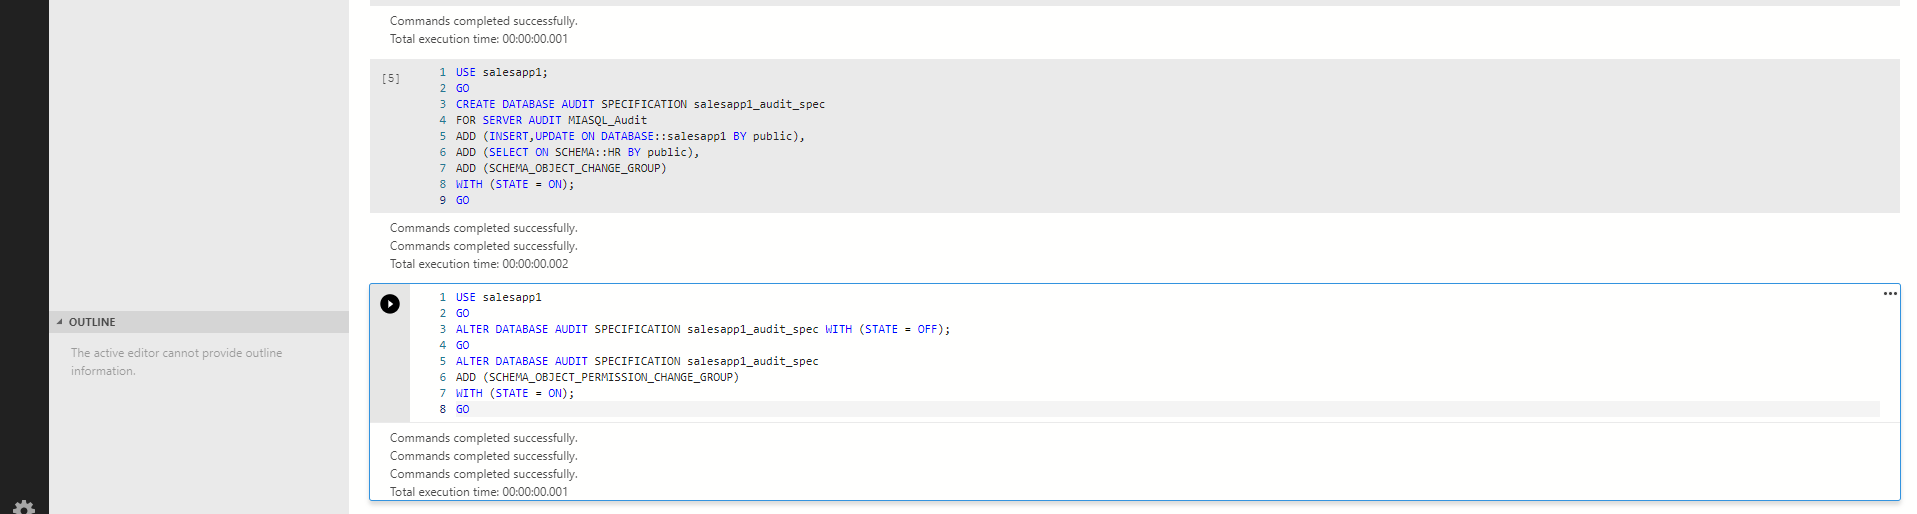
\includegraphics[width=16cm, height=90]{./Imagenes/Imagen_15}
   				    \end{center}
   				    
   	      
   	      \item Paso 6 Examinar metadatos de auditoría
				 
				 	
					\begin{center}
    				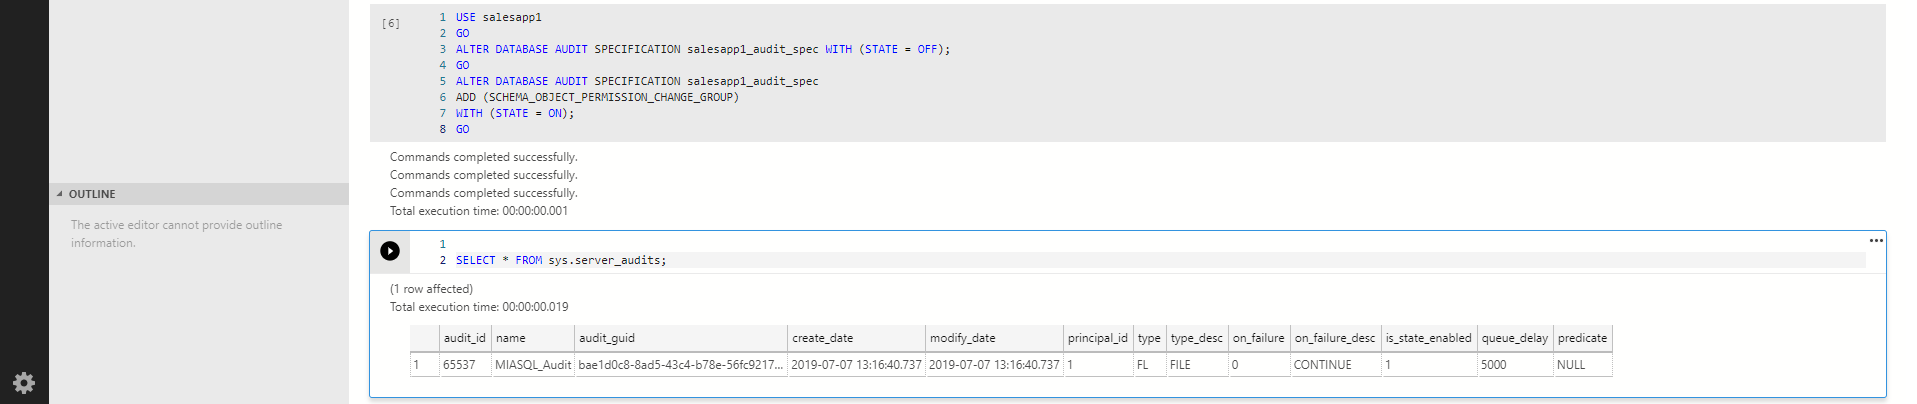
\includegraphics[width=16cm, height=90]{./Imagenes/Imagen_16}
   				    \end{center}
   				    
   	      \item Paso 7 Examinar los metadatos de especificación de auditoría del servidor
				 
				 	
					\begin{center}
    				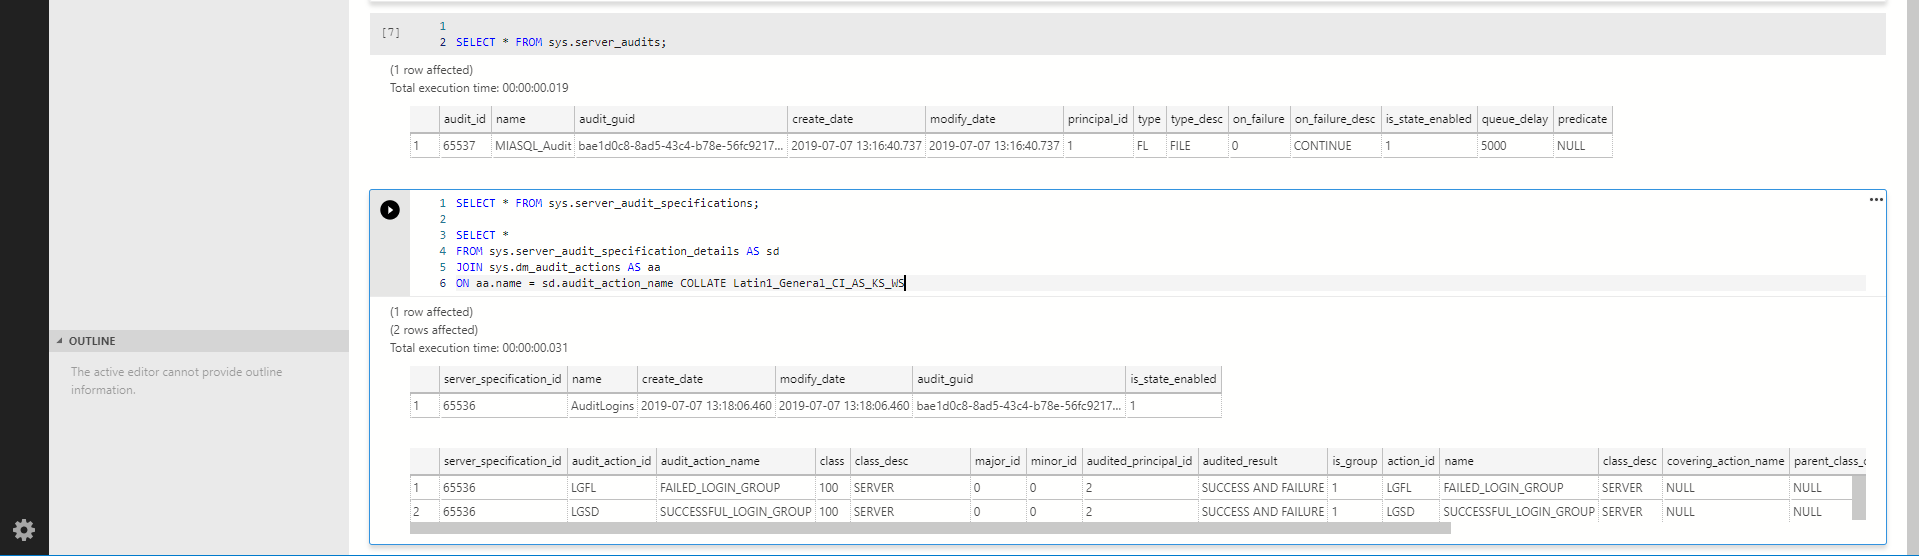
\includegraphics[width=16cm, height=90]{./Imagenes/Imagen_17}
   				    \end{center}
   				    
   	      \item Paso 8 Examinar los metadatos de especificación de auditoría de base de datos
				 
				 	
					\begin{center}
    				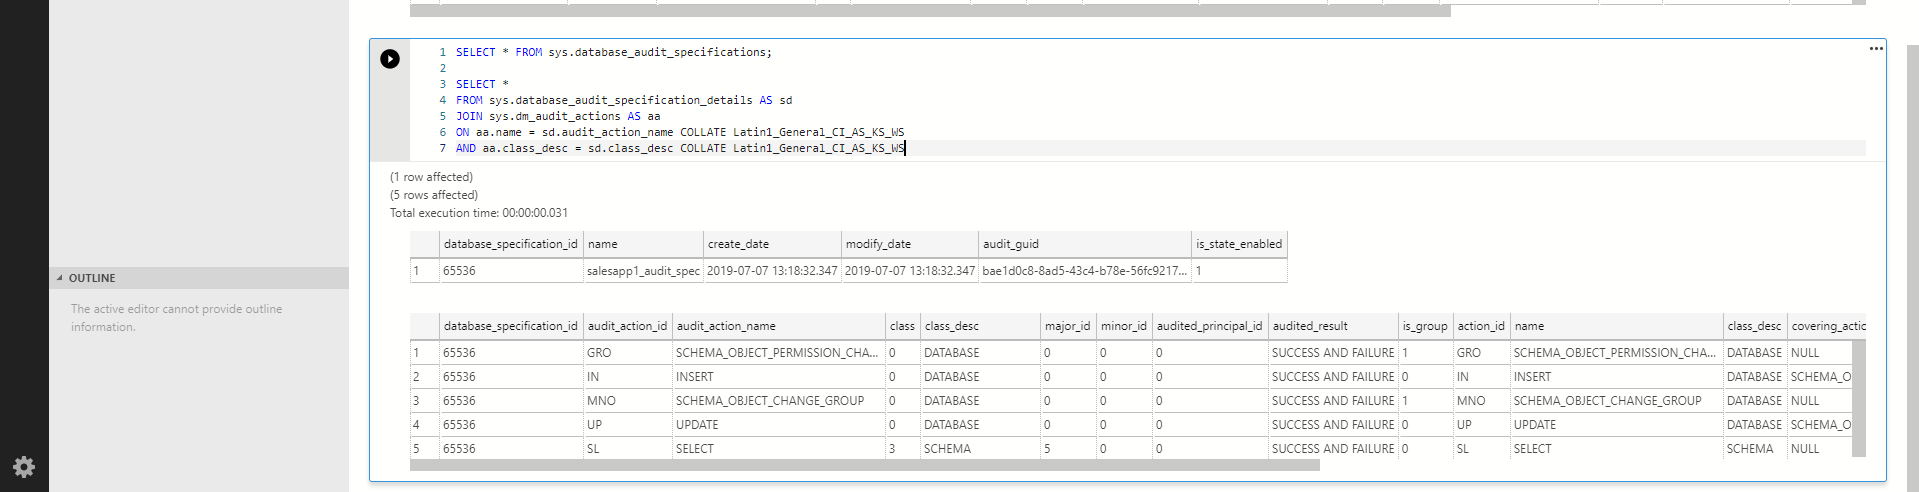
\includegraphics[width=16cm, height=90]{./Imagenes/Imagen_18}
   				    \end{center}
   				    
   		   \item Paso 9 quitar la auditoria
				 
				 	
					\begin{center}
    				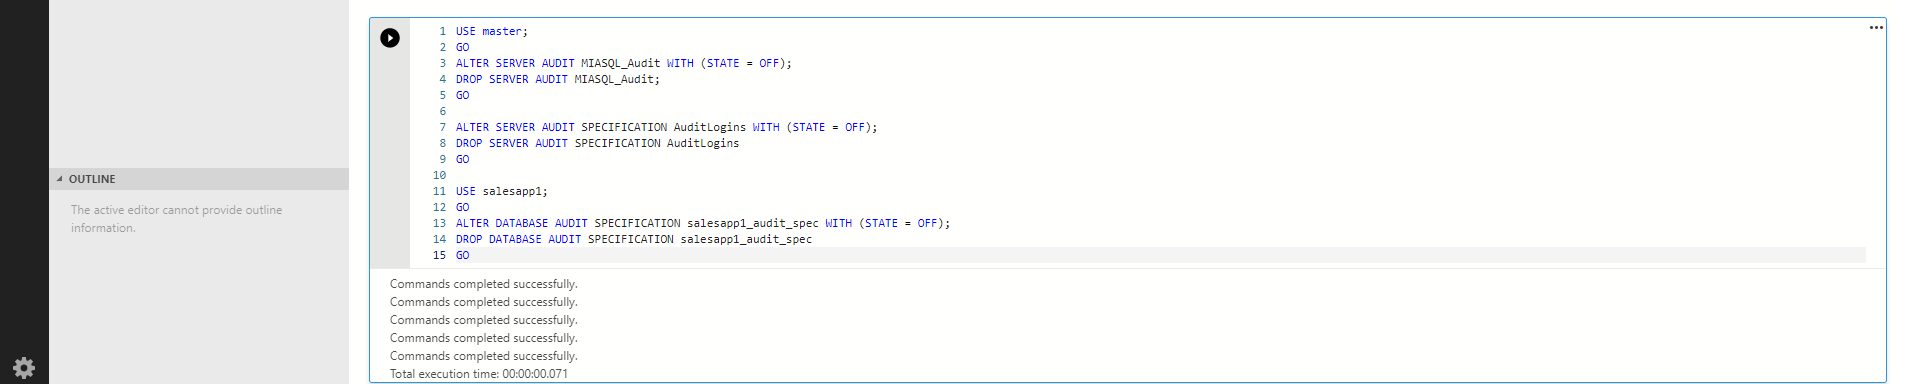
\includegraphics[width=16cm, height=90]{./Imagenes/Imagen_19}
   				    \end{center}
   				    
   		   \end{itemize}
				    \clearpage	
				    
				    
\subsection{Ejercicio N° 03: Utilizando auditorías personzalizadas}

\begin{itemize}  


			\item Paso 1 Crear una auditoria
				 
				 	
					\begin{center}
    				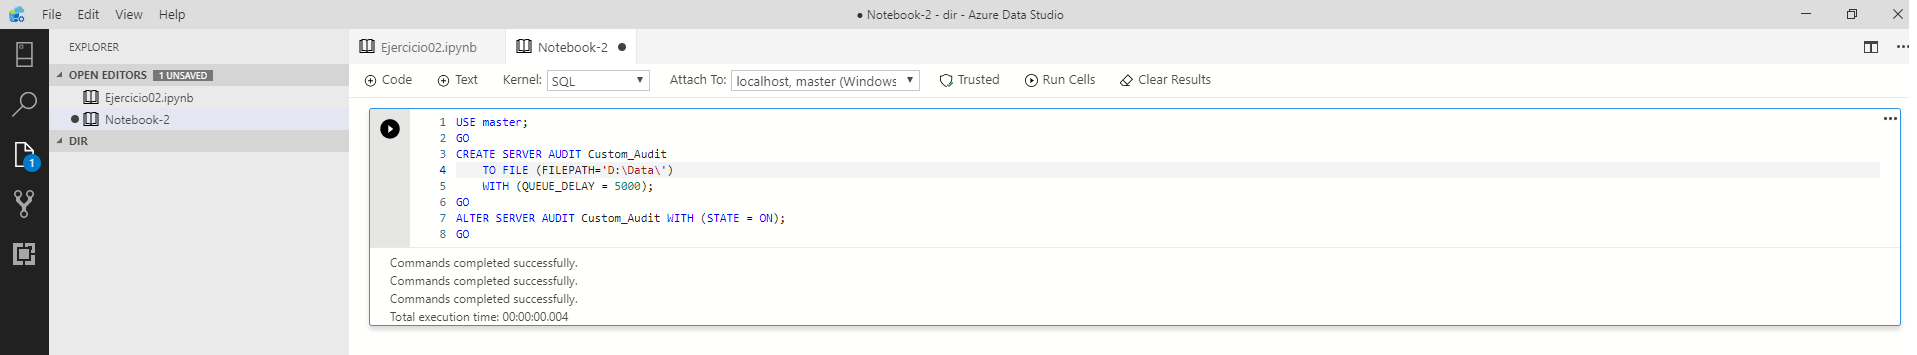
\includegraphics[width=16cm, height=90]{./Imagenes/Imagen__20}
   				    \end{center}
   				    
   				     \begin{center}
    				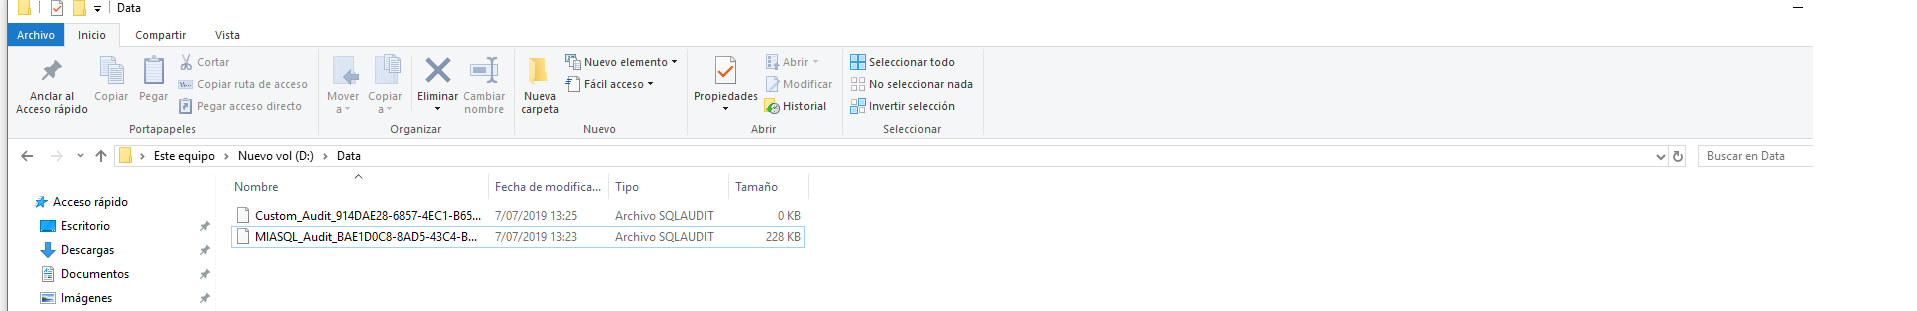
\includegraphics[width=16cm, height=90]{./Imagenes/AuditoriaCreada2}
   				    \end{center}
   				    
   		   \item Paso 2 crear una especificación de auditoría del servidor que incluya el grupo de acción USER DEFINED AUDIT GROUP
				 
				 	
					\begin{center}
    				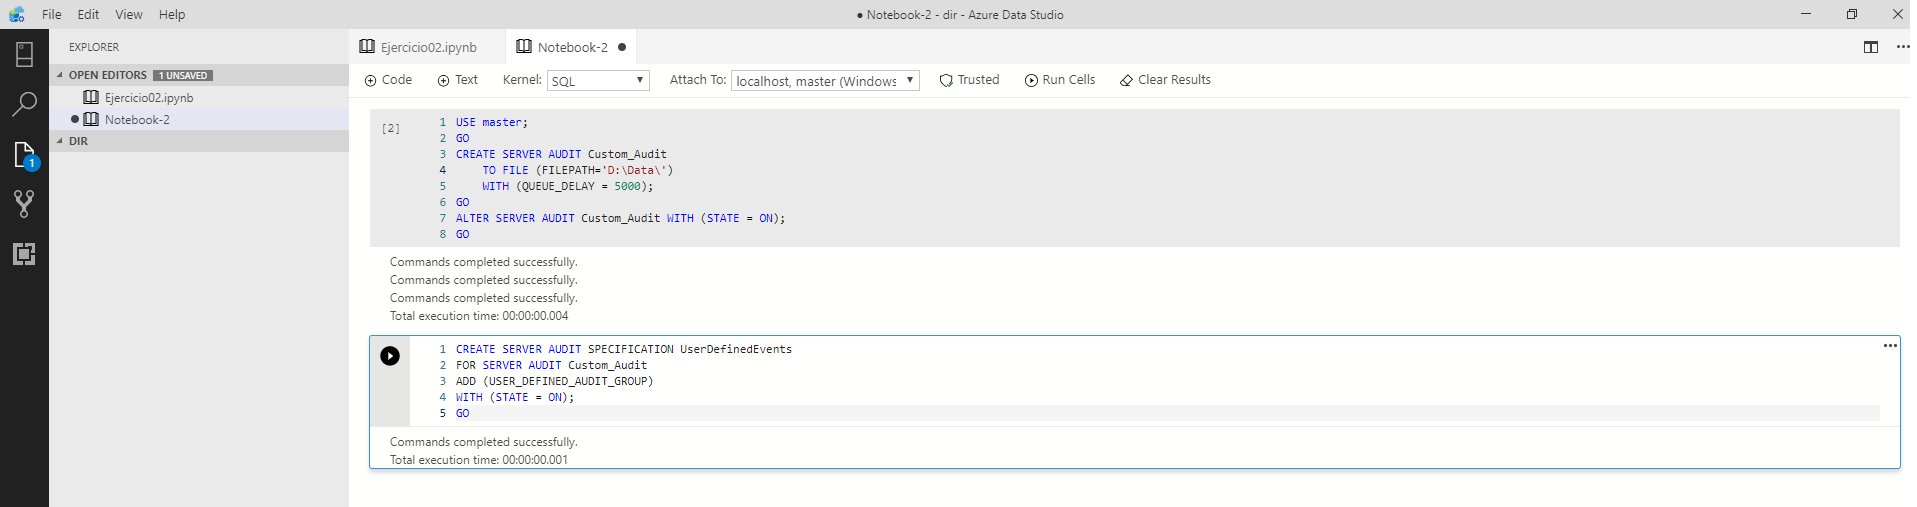
\includegraphics[width=16cm, height=90]{./Imagenes/Imagen__21}
   				    \end{center}
   				    
   		   \item Paso 3 llama a sp audit write directamente
				 
				 	
					\begin{center}
    				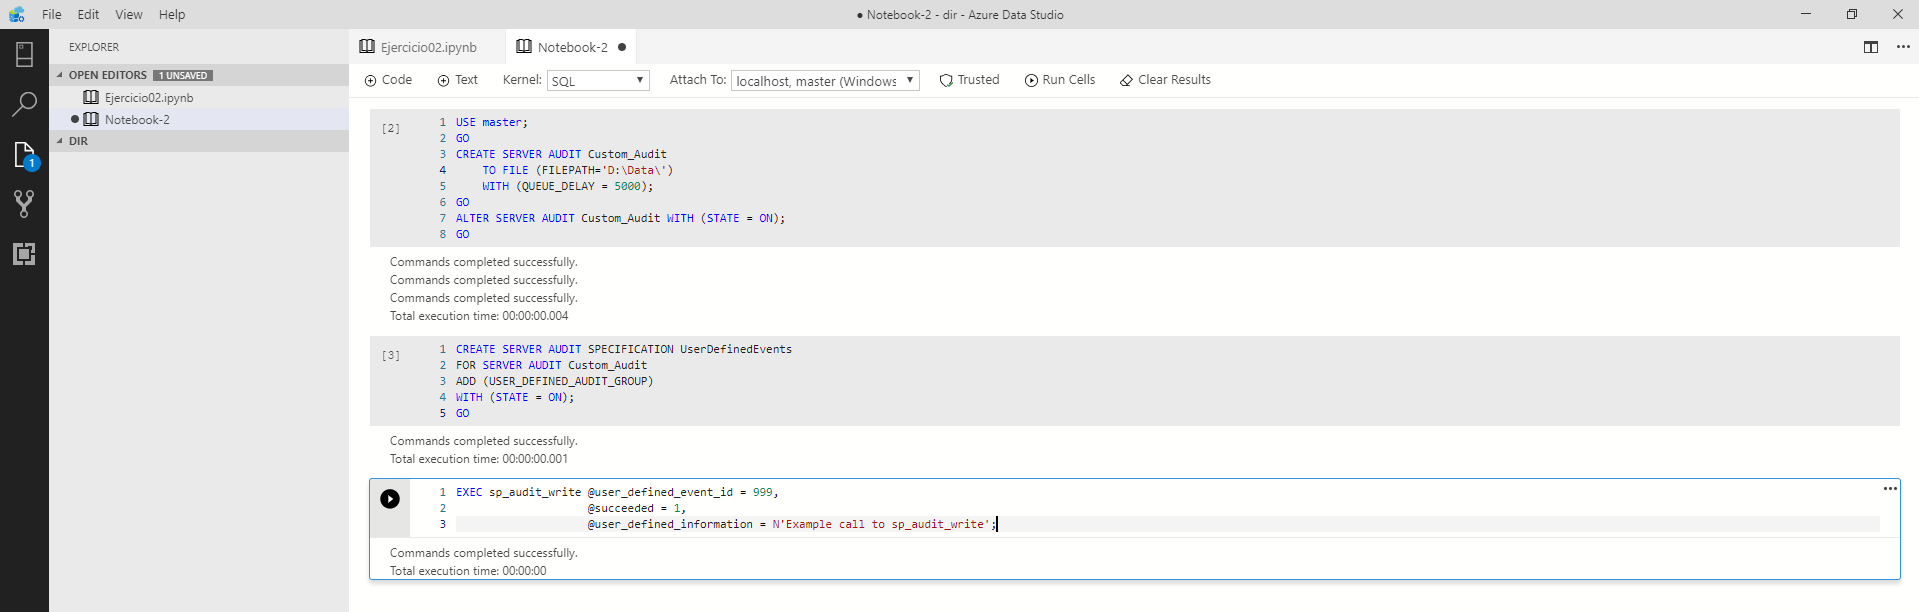
\includegraphics[width=16cm, height=90]{./Imagenes/Imagen__22}
   				    \end{center}
   				    
   		   \item Paso 4 Demostrar cómo aparece un evento personalizado en la auditoría.
				 
				 	
					\begin{center}
    				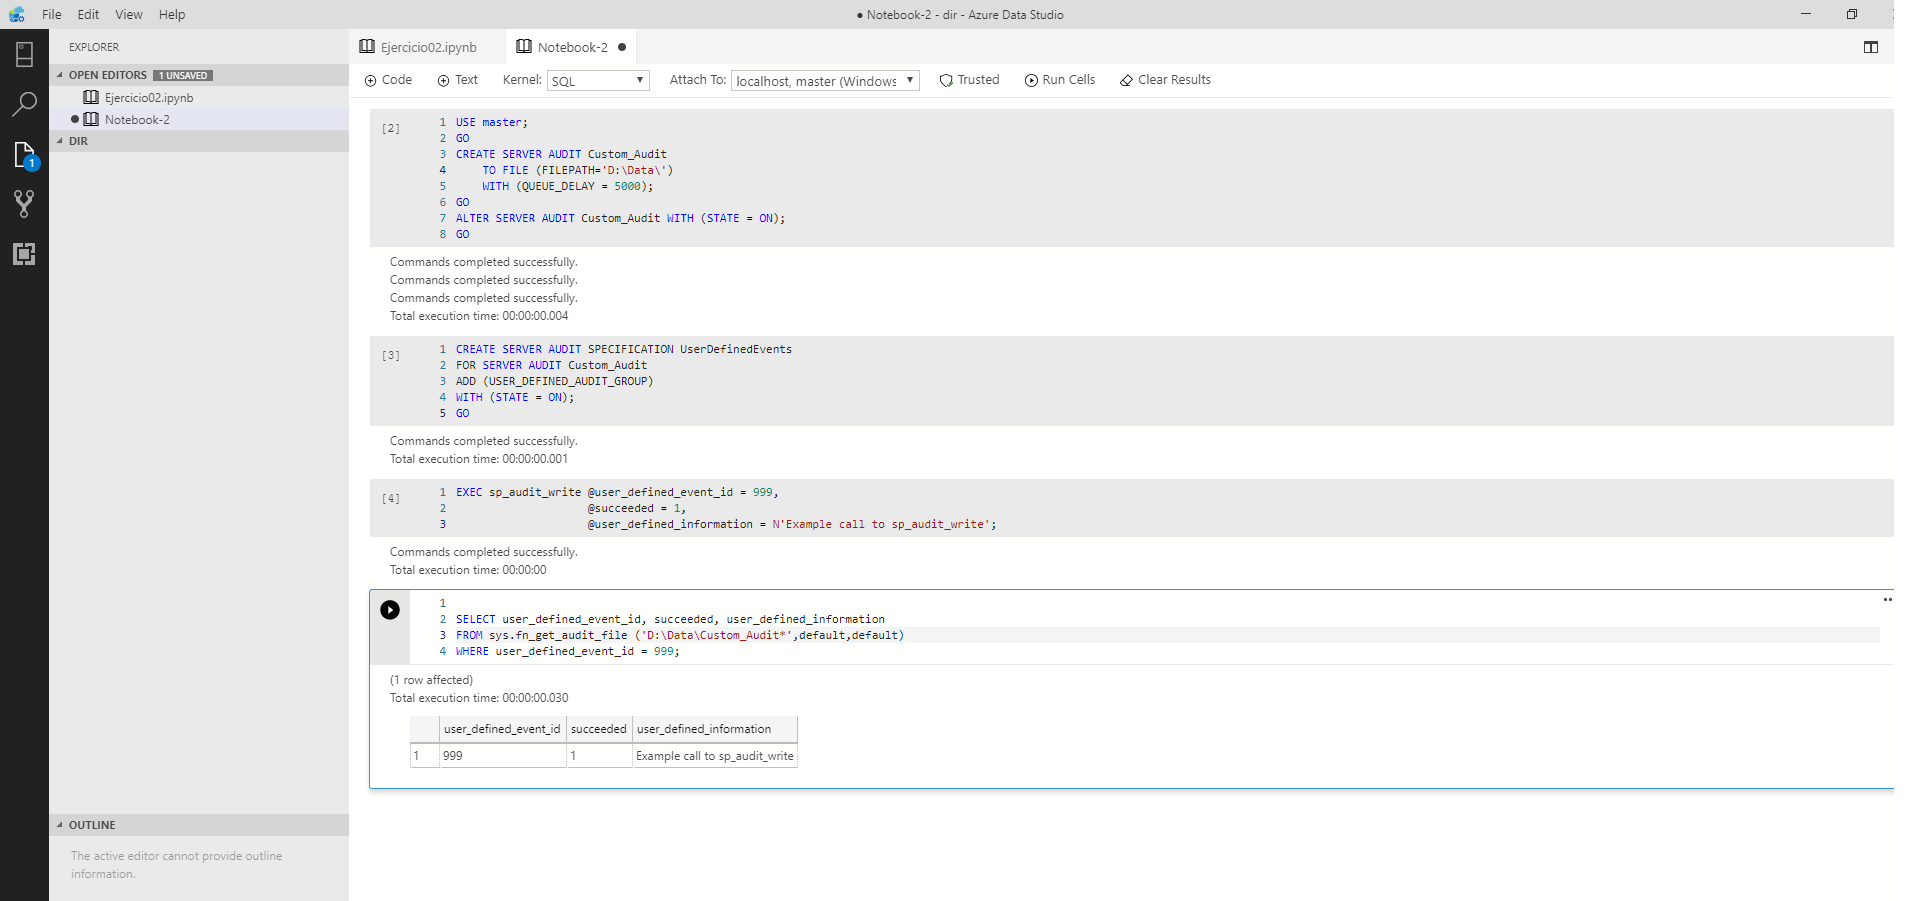
\includegraphics[width=16cm, height=90]{./Imagenes/Imagen__23}
   				    \end{center}
   				    
   		  \item Paso 5 demostrar el uso de sp audit write en un procedimiento almacenado
				 
				 	
					\begin{center}
    				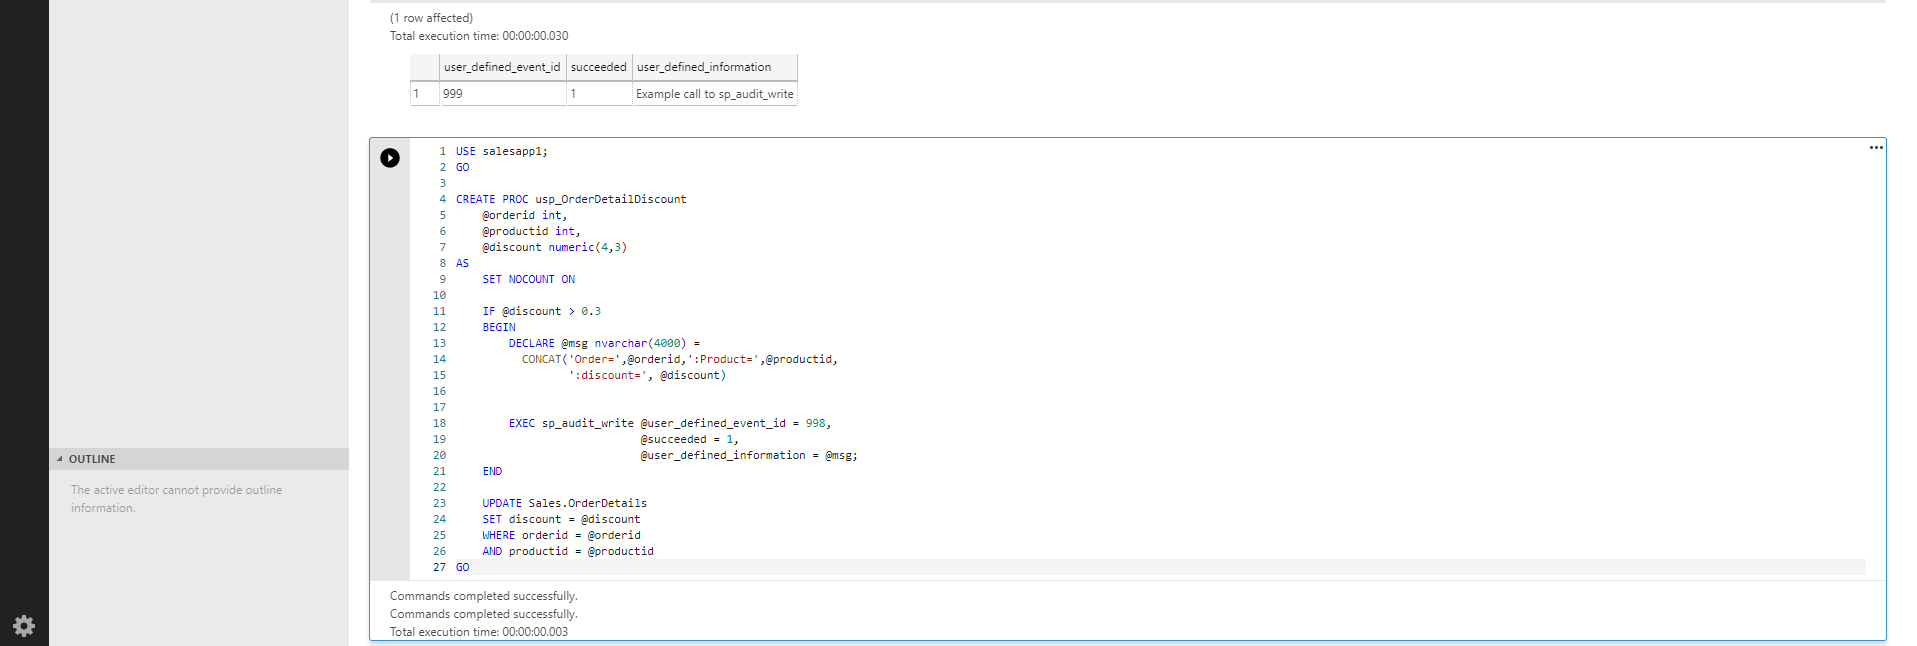
\includegraphics[width=16cm, height=90]{./Imagenes/Imagen__24}
   				    \end{center}
   				    
   	      
   	      \item Paso 6 llame al procedimiento almacenado dos veces La primera llamada no debe generar un evento de auditoría personalizado La segunda llamada debe generar un evento de auditoría personalizado
				 
				 	
					\begin{center}
    				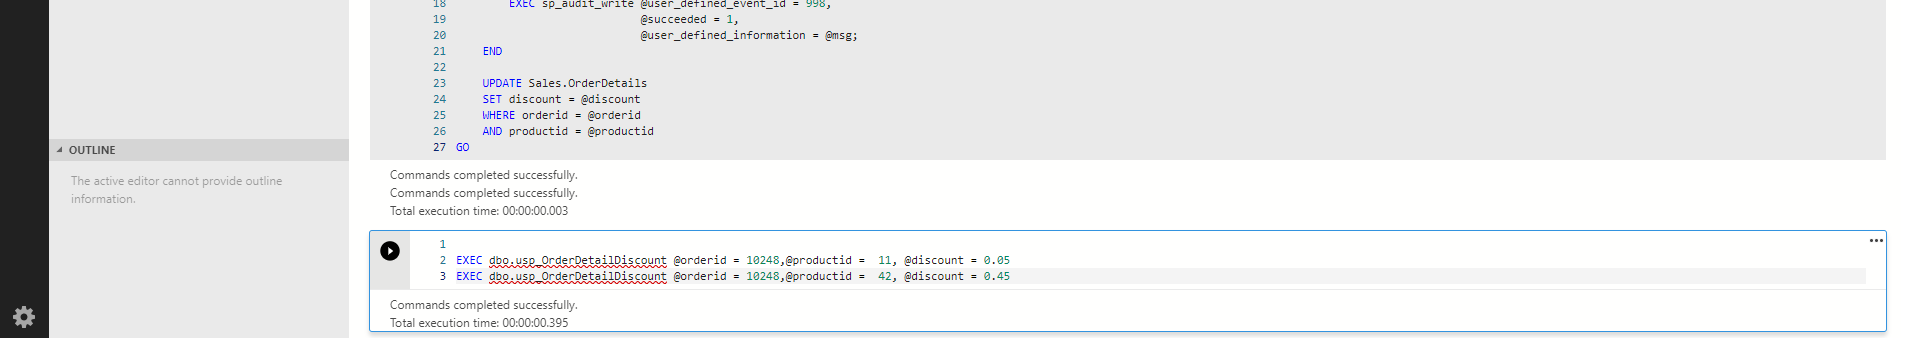
\includegraphics[width=16cm, height=90]{./Imagenes/Imagen__25}
   				    \end{center}
   				    
   	      \item Paso 7 examinar los datos de auditoría
				 
				 	
					\begin{center}
    				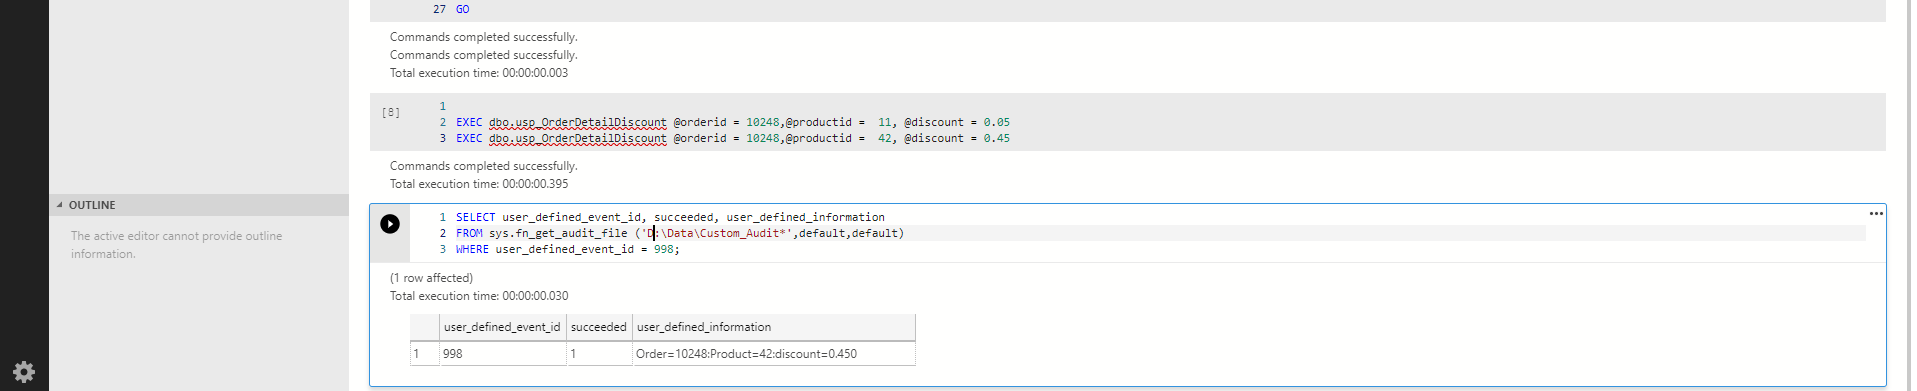
\includegraphics[width=16cm, height=90]{./Imagenes/Imagen__26}
   				    \end{center}
   				    
   	      \item Paso 8 abandonar la auditoria
				 
				 	
					\begin{center}
    				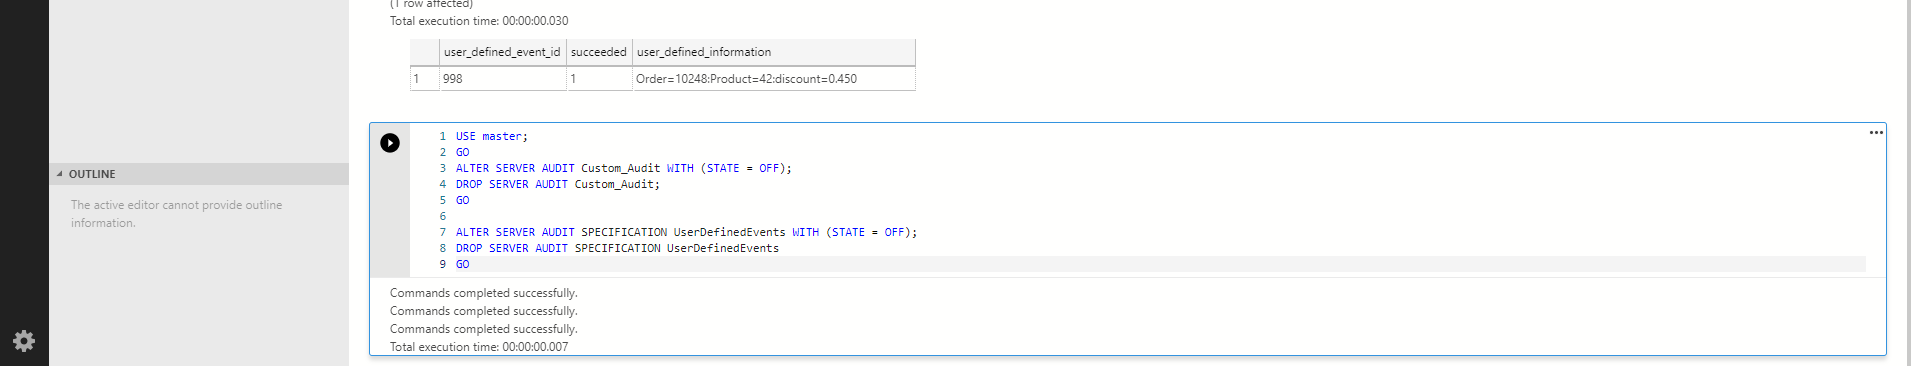
\includegraphics[width=16cm, height=90]{./Imagenes/Imagen__27}
   				    \end{center}
   				    
   		   


\end{itemize}
\clearpage	

\subsection{Ejercicio N° 04: Administrando auditorías}
\begin{itemize}


			
			\item Paso 1 crear una auditoría con un archivo de destino
				 
				 	
					\begin{center}
    				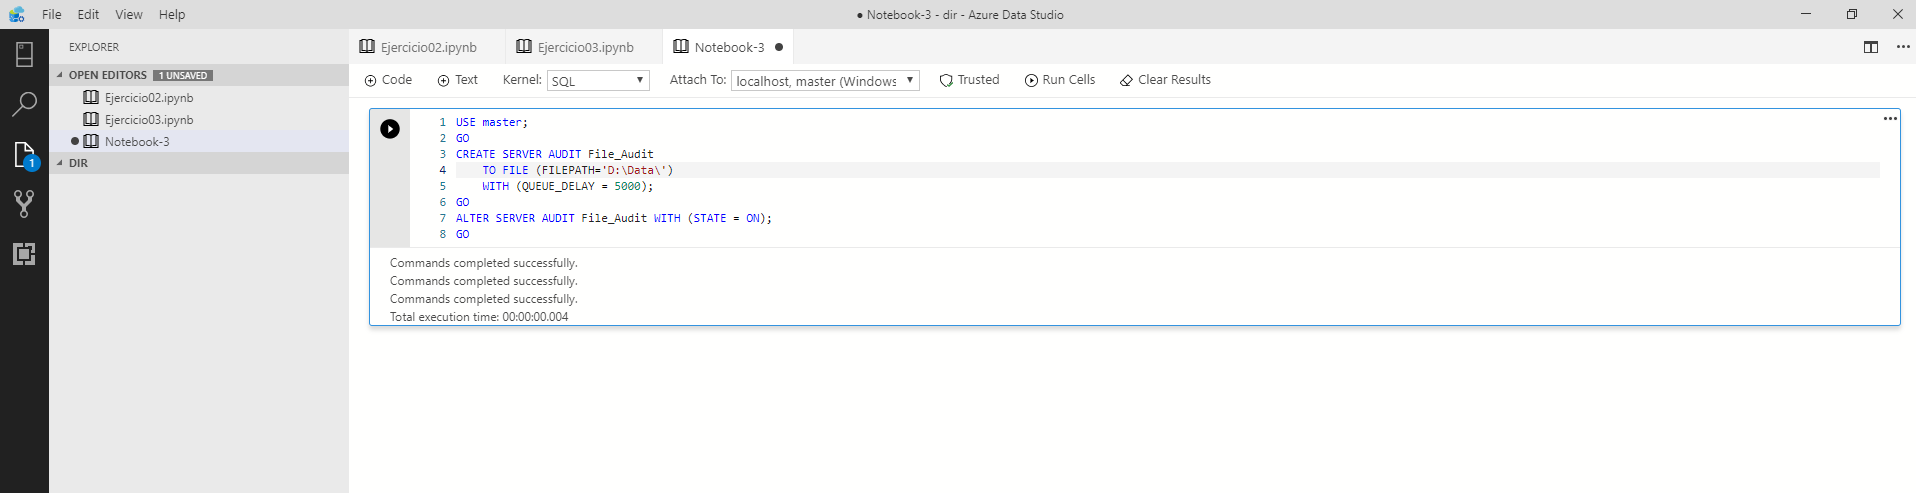
\includegraphics[width=16cm, height=90]{./Imagenes/ImagenlV28}
   				    \end{center}
   				    
   				     \begin{center}
    				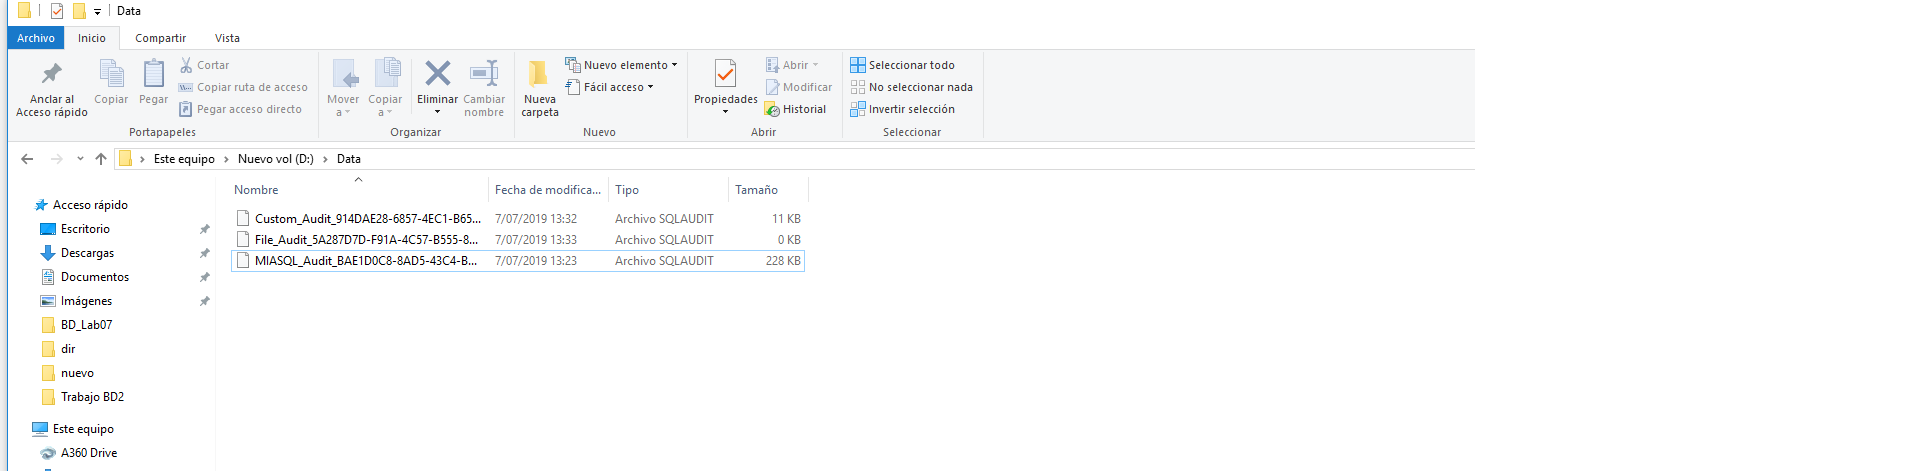
\includegraphics[width=16cm, height=90]{./Imagenes/AuditoriaCreada3}
   				    \end{center}
   				    
   		   \item Paso 2 crear una auditoría con un destino de registro de aplicación de Windows
				 
				 	
					\begin{center}
    				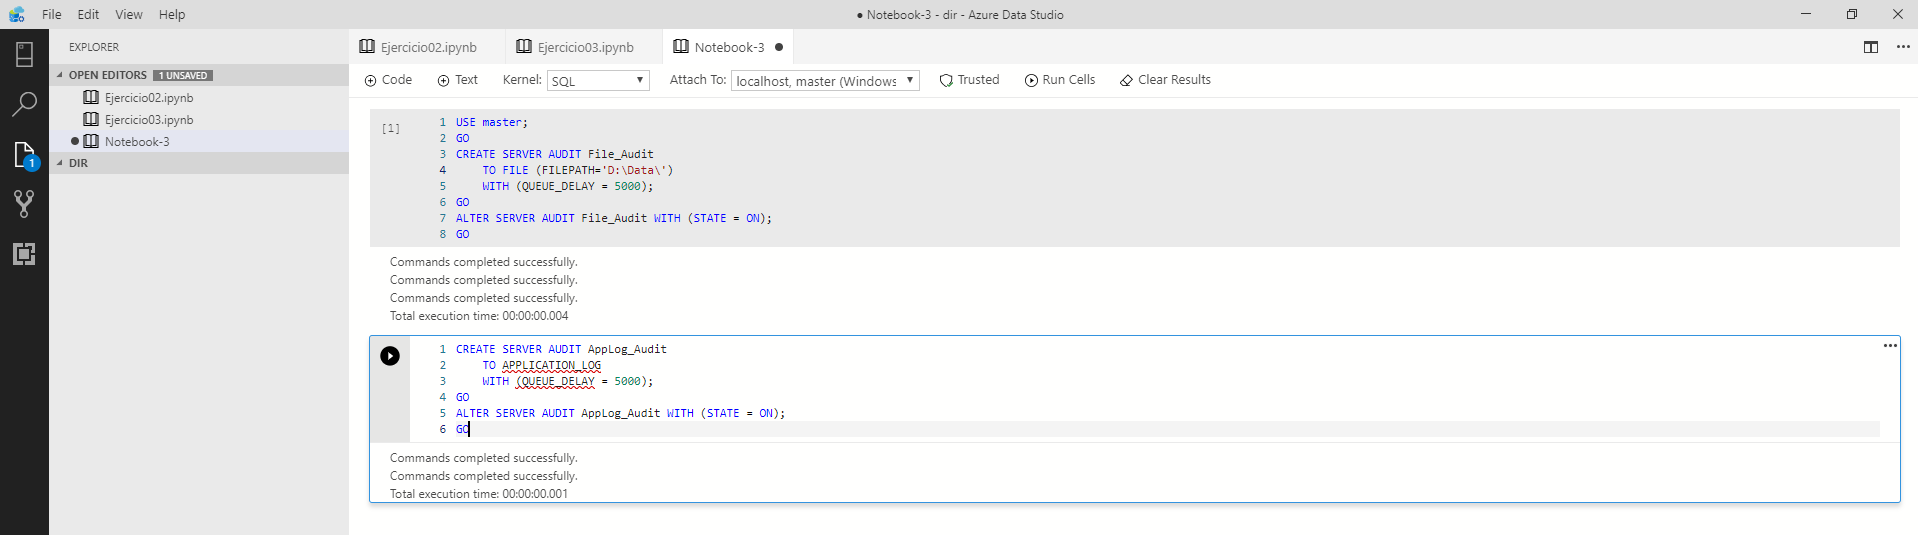
\includegraphics[width=16cm, height=90]{./Imagenes/ImagenlV29}
   				    \end{center}
   				    
   		   \item Paso 3 agregar la misma especificación de auditoría de base de datos a ambas auditorías
				 
				 	
					\begin{center}
    				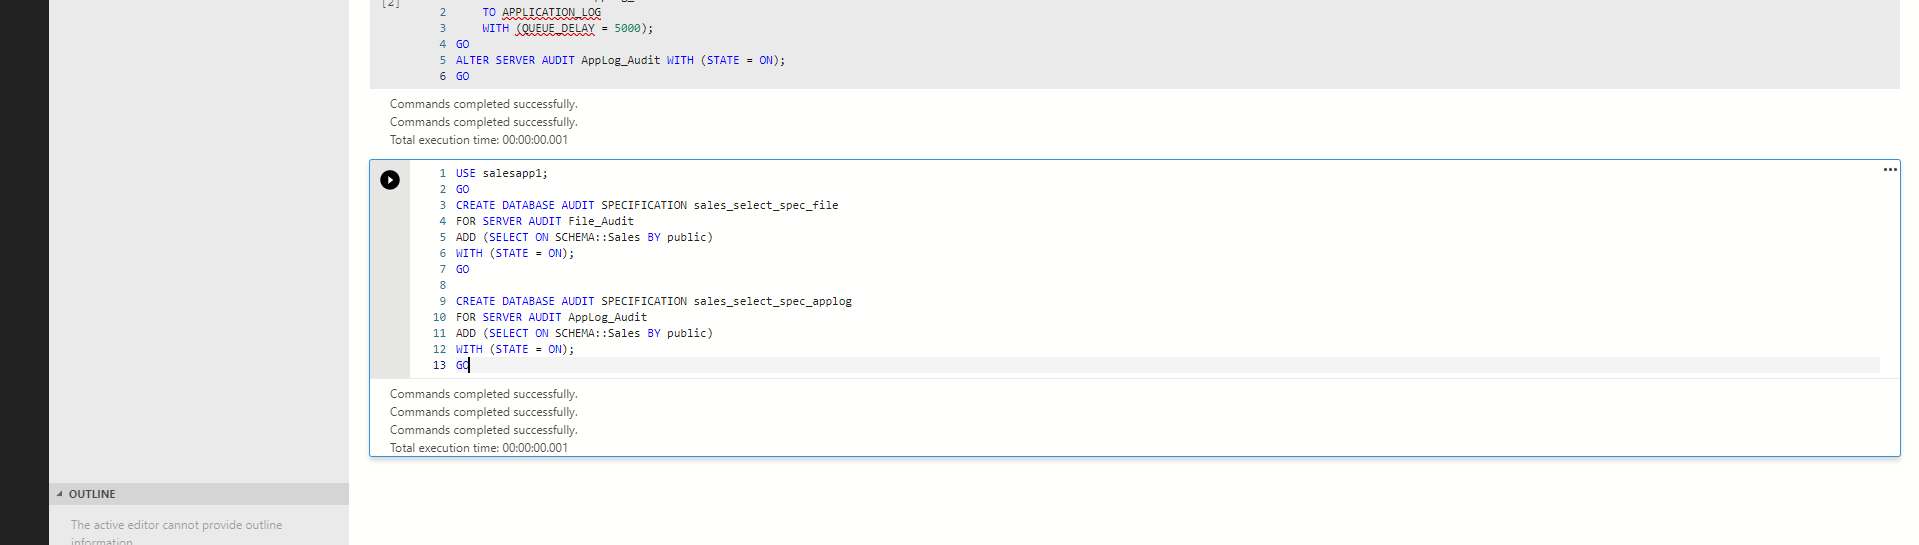
\includegraphics[width=16cm, height=90]{./Imagenes/ImagenlV30}
   				    \end{center}
   				    \clearpage				
   		   \item Paso 4 Ejecutar una instrucción de selección simple que coincida con la especificación de auditoría
				 
				 	
					\begin{center}
    				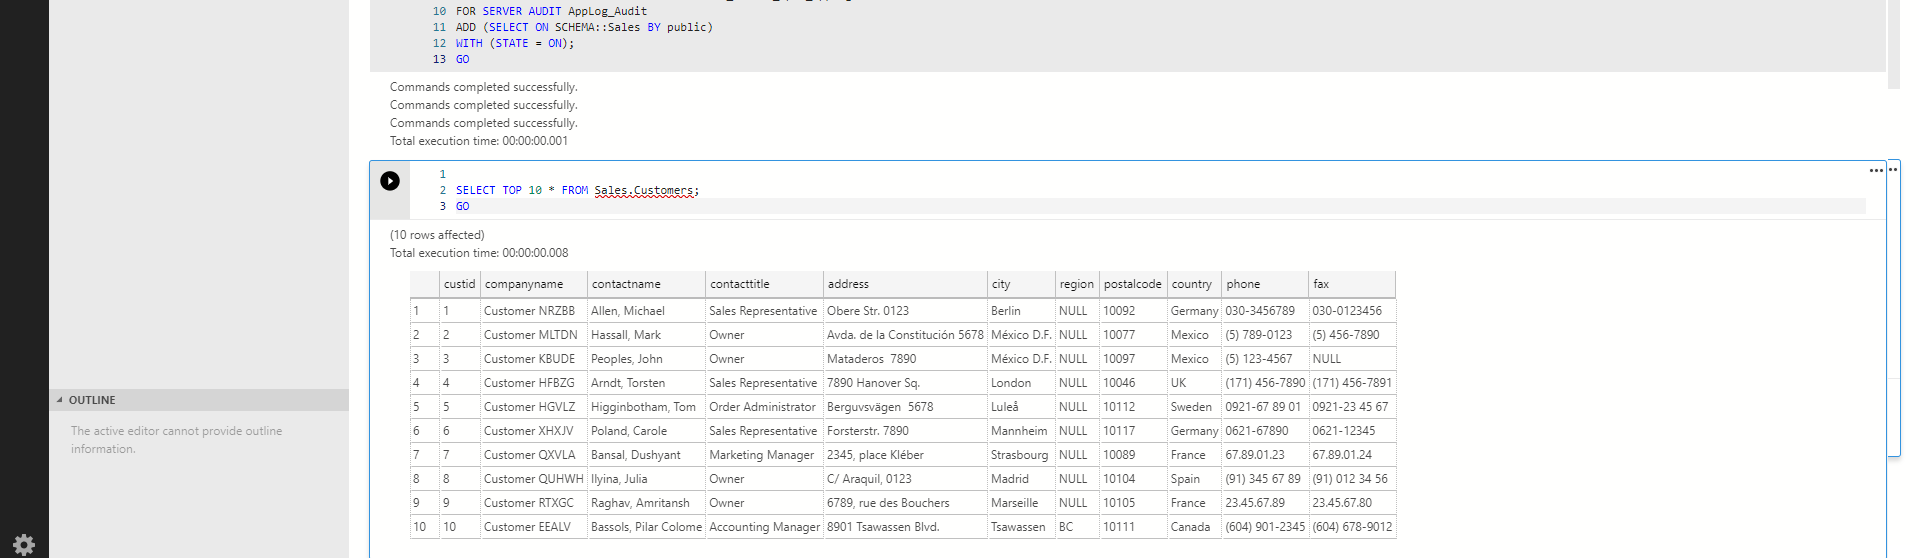
\includegraphics[width=16cm, height=90]{./Imagenes/ImagenlV31}
   				    \end{center}
   				    
   		  \item Paso 5 Examine la salida de auditoría basada en archivos. Demostrar algunos de los campos más útiles.
				 
				 	
					\begin{center}
    				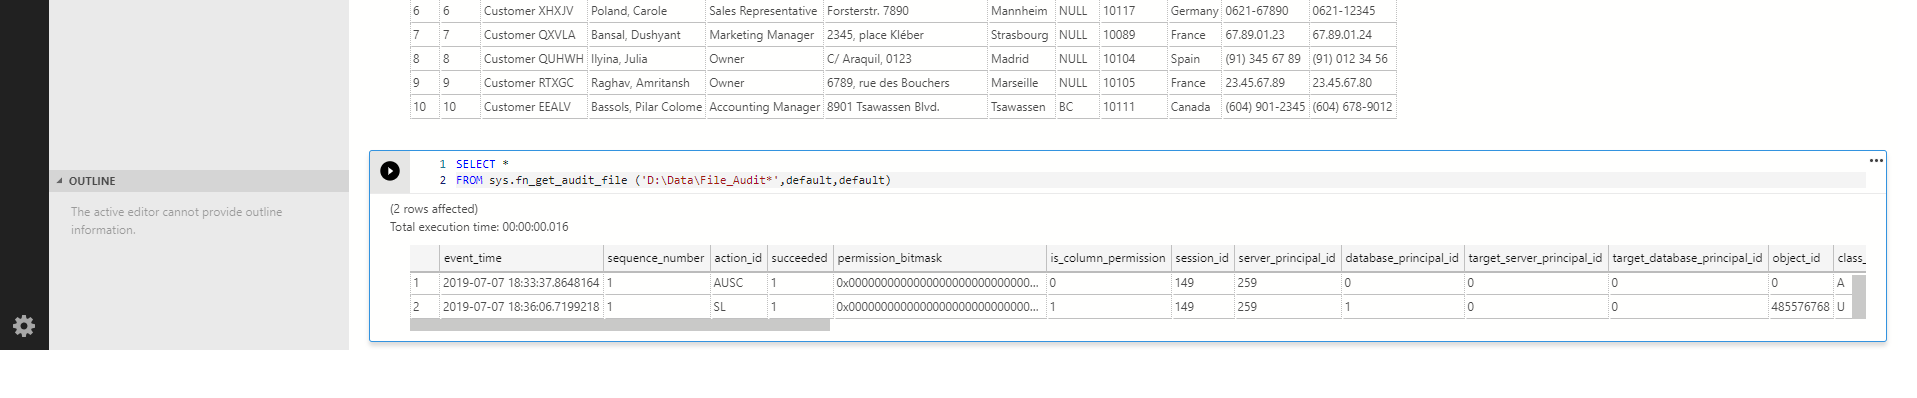
\includegraphics[width=16cm, height=90]{./Imagenes/ImagenlV32}
   				    \end{center}
   				    
   	      
   	      \item Paso 6 examinar la salida de auditoría de registro de aplicación de Windows. Usar el visor de eventos
				 
				 	
					\begin{center}
    				\includegraphics[width=16cm, height=90]{./Imagenes/Imagen}
   				    \end{center}
   				    
   	      \item Paso 7 abandone las auditorías y las especificaciones de auditoría, tenga en cuenta que las auditorías y las especificaciones deben desactivarse antes de poder retirarse
				 
				 	
					\begin{center}
    				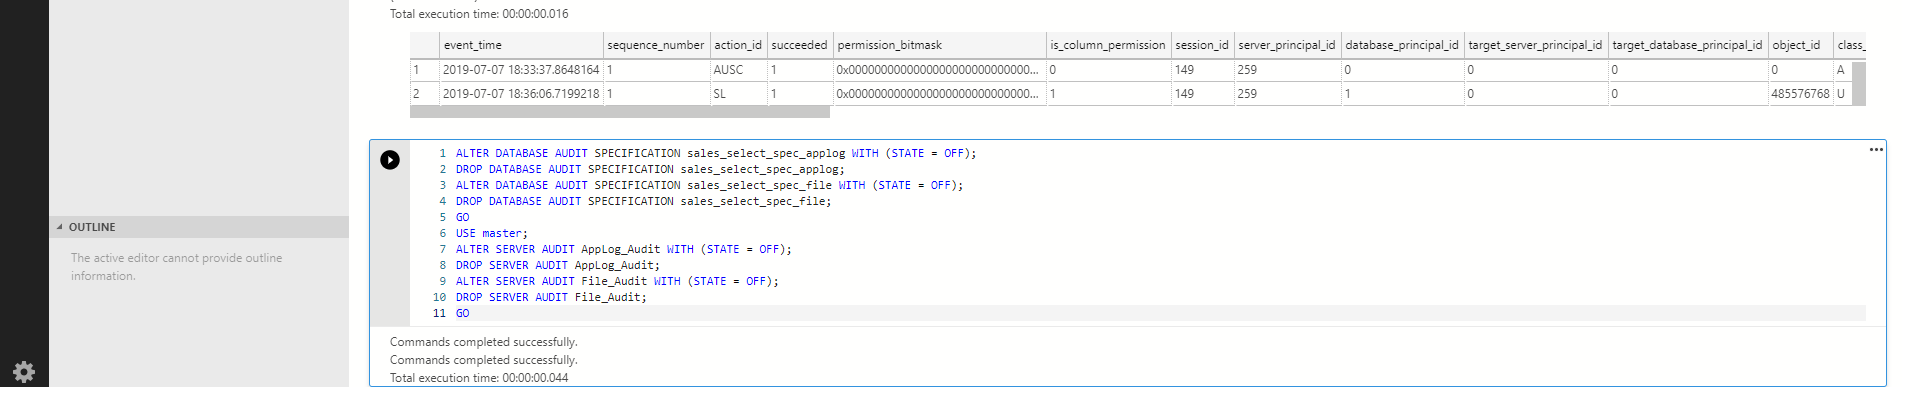
\includegraphics[width=16cm, height=90]{./Imagenes/ImagenlV33}
   				    \end{center}
   				    
\end{itemize}
\clearpage	
			

\\\\




